\RequirePackage{ifpdf}
\documentclass[phd,tocprelim]{cornell}
%
% tocprelim option must be included to put the roman numeral pages in the
% table of contents
%
% The cornellheadings option will make headings completely consistent with
% guidelines.
%
% This sample document was originally provided by Blake Jacquot, and
% fixed up by Andrew Myers.
%

% AMS
\usepackage{amsmath}
\usepackage{amsopn} 
\usepackage{amssymb}
\usepackage{amsthm}

% Graphics
\usepackage{adjustbox}
\usepackage{float}
\usepackage{graphicx,pstricks}
\usepackage{graphics}
\usepackage{subfigure}
\usepackage{epsfig}

% Bibtex
\usepackage[numbers,compress]{natbib}

% Algorithm
\usepackage[ruled]{algorithm2e}

% Others
\usepackage{accents} 
\usepackage{bm}
\usepackage{booktabs}
\usepackage[format=hang]{caption}
\usepackage{colortbl}
\usepackage{enumitem}
\usepackage[OT1]{fontenc}
\usepackage{hyphenat}
\usepackage{lineno}
\usepackage{moreverb}
\usepackage{multirow} 
\usepackage{nicefrac}
\usepackage[refpage,intoc]{nomencl}
\usepackage{palatino}
\usepackage{placeins}
\usepackage{siunitx}
\usepackage{threeparttable}
\usepackage{txfonts}
\usepackage{url}
\usepackage{xcolor}
\usepackage[pageanchor, hidelinks]{hyperref}
\def\pagedeclaration#1{\dotfill\hyperlink{page.#1}{Page\nobreakspace#1}}
\setlength{\nomitemsep}{-\parsep}

\definecolor{lightgray}{rgb}{0.83, 0.83, 0.83}

%if you're having problems with overfull boxes, you may need to increase
%the tolerance to 9999
\tolerance=9999

\bibliographystyle{plain}
%\bibliographystyle{IEEEbib}

% \renewcommand{\caption}[1]{\singlespacing\hangcaption{#1}\normalspacing}
\renewcommand{\topfraction}{0.85}
\renewcommand{\textfraction}{0.1}
\renewcommand{\floatpagefraction}{0.75}

% Add the notation used in this thesis
% Math Bold
\newcommand{\Bb}{\bm{b}}
\newcommand{\Bc}{\bm{c}}
\newcommand{\Bd}{\bm{d}}
\newcommand{\Be}{\bm{e}}
\newcommand{\Bh}{\bm{h}}
\newcommand{\Bhhat}{\smash{\hat{\bm{h}}}}
\newcommand{\Br}{\bm{r}}
\newcommand{\Brhat}{\smash{\hat{\bm{r}}}}
\newcommand{\Bu}{\bm{u}}
\newcommand{\Bw}{\bm{w}}
\newcommand{\Bx}{\bm{x}}
\newcommand{\By}{\bm{y}}
\newcommand{\Bz}{\bm{z}}
\newcommand{\BA}{\bm{A}}
\newcommand{\BB}{\bm{B}}
\newcommand{\BBreve}{\smash{\breve{\bm{B}}}}
\newcommand{\BC}{\bm{C}}
\newcommand{\BCbar}{\overline{\bm{C}}}
\newcommand{\BD}{\bm{D}}
\newcommand{\BE}{\bm{E}}
\newcommand{\BH}{\bm{H}}
\newcommand{\BHhat}{\smash{\hat{\bm{H}}}}
\newcommand{\BHdiag}{\smash{\hat{\bm{H}}_{diag}}}
\newcommand{\BI}{\bm{I}}
\newcommand{\BP}{\bm{P}}
\newcommand{\BQ}{\bm{Q}}
\newcommand{\BR}{\bm{R}}
\newcommand{\BS}{\bm{S}}
\newcommand{\BT}{\bm{T}}
\newcommand{\BU}{\bm{U}}
\newcommand{\BV}{\bm{V}}
\newcommand{\BW}{\bm{W}}
\newcommand{\BX}{\bm{X}}
\newcommand{\BXbar}{\overline{\bm{X}}}
\newcommand{\BY}{\bm{Y}}
\newcommand{\BYbar}{\overline{\bm{Y}}}
\newcommand{\BZ}{\bm{Z}}
\newcommand{\BZtilde}{\widetilde{\bm{Z}}}

\newcommand{\Balpha}{\bm{\alpha}}
\newcommand{\Btheta}{\bm{\theta}}
\newcommand{\Bzeta}{\bm{\zeta}}
\newcommand{\BLambda}{\bm{\Lambda}}
\newcommand{\BPhi}{\bm{\Phi}}
\newcommand{\BPi}{\bm{\Pi}}
\newcommand{\BTheta}{\bm{\Theta}}

\newcommand{\BfX}{\bm{f_X}}
\newcommand{\BmuX}{\bm{\mu_X}}
\newcommand{\BK}[1]{\bm{K_{#1}}}
\newcommand{\BKtil}[1]{\bm{\tilde{K}_{#1}}}
% \newcommand{\BKtil}[1]{\tilde{\bm{K}}_{\!\textit{\textbf{#1}}}}

% Math Blackboard Bold
\newcommand{\BBR}{\mathbb{R}}

% Math Relation
\newcommand{\Eq}{\mathrel{=}}
\newcommand{\Minus}{\mathrel{-}}
\newcommand{\Plus}{\mathrel{+}}

% Math Binary
\newcommand{\binsubset}{\mathbin{\subset}}
\newcommand{\Colon}{\mathbin{:}}
\newcommand{\Geq}{\mathbin{\geq}}
\newcommand{\Leq}{\mathbin{\leq}}
\newcommand{\Sim}{\mathbin{\sim}}
\newcommand{\Times}{\mathbin{\times}}
\newcommand{\To}{\mathbin{\to}}

% Math Calligraphy
\newcommand{\calC}{\mathcal{C}}
\newcommand{\calL}{\mathcal{L}}
\newcommand{\calN}{\mathcal{N}}
\newcommand{\calO}{\mathcal{O}}
\newcommand{\NN}{\mathcal{NN}}
\newcommand{\NOR}{\mathcal{NOR}}
\newcommand{\PSD}{\mathcal{PSD}}
\newcommand{\GP}{\mathcal{GP}}
\newcommand{\calo}{\mathchoice
	{{\scriptstyle\mathcal{O}}}% \displaystyle
	{{\scriptstyle\mathcal{O}}}% \textstyle
	{{\scriptscriptstyle\mathcal{O}}}% \scriptstyle
	{\scalebox{.6}{$\scriptscriptstyle\mathcal{O}$}}%\scriptscriptstyle
}

% Math Operator
\DeclareMathOperator*{\argmax}{arg\,max}
\DeclareMathOperator*{\argmin}{arg\,min}
\DeclareMathOperator{\diag}{diag}
\DeclareMathOperator{\dist}{dist}
\DeclareMathOperator{\dx}{\partial\!}
\DeclareMathOperator{\ddx}{\partial^2\!}
\DeclareMathOperator{\tr}{tr}
\DeclareMathOperator{\vol}{vol}
\DeclareMathOperator{\BBE}{\mathbb{E}}
\DeclareMathOperator{\In}{\in}
\DeclareMathOperator{\Lip}{Lip}
\DeclareMathOperator{\Proj}{Proj}
\DeclareMathOperator{\Ref}{ref}
\DeclareMathOperator{\Sec}{s}
\DeclareMathOperator{\SoR}{SoR}
\DeclareMathOperator{\Span}{Span}
\DeclareMathOperator{\Var}{Var}
\newcommand{\abs}[1]{\left\lvert#1\right\rvert}
\newcommand{\norm}[1]{\left\lVert#1\right\rVert}

% Graph

\newcommand{\Erdos}{Erd\H{o}s}
\newcommand{\ErdosRenyi}{Erd\H{o}s-R\'enyi}

% Gaussian Processes
\newcommand{\K}[1]{K_{#1}}
\newcommand{\Ktil}[1]{\tilde{K}_{#1}}
\DeclareMathOperator{\mile}{mile}

% Chemistry Unit
\DeclareMathOperator{\au}{au}
\DeclareMathOperator{\Ha}{Ha}
\DeclareMathOperator{\HaPA}{\si{Ha/atom}}
\DeclareMathOperator{\HaPB}{\si{Ha/Bohr}}
\DeclareMathOperator{\HaPps}{\si{Ha/ps}}
\DeclareMathOperator{\Kelvin}{K}

% Helper Command
\newcommand{\numintitle}[1]{\texorpdfstring{#1}{}}
\newcommand{\ph}{\phantom{ }}

% Color
\definecolor{burgundy}{RGB}{140,0,26}

% Environment
\newcommand{\algorithmnormal}[1]{
	\begin{algorithm}
		\normalspacing{
			#1
		}
	\end{algorithm}
}

% Define theorem environment
% Defintions, theorems, etc
\usepackage[framemethod=tikz, nobreak = true]{mdframed}
\newmdtheoremenv{theorem}{Theorem}
\AtBeginEnvironment{theorem}{\begin{minipage}{\textwidth}}
\AtEndEnvironment{theorem}{\end{minipage}}

\newmdtheoremenv{definition}{Definition}
\AtBeginEnvironment{definition}{\begin{minipage}{\textwidth}}
\AtEndEnvironment{definition}{\end{minipage}}

\newmdtheoremenv{claim}[theorem]{Claim}
\AtBeginEnvironment{claim}{\begin{minipage}{\textwidth}}
\AtEndEnvironment{claim}{\end{minipage}}

\newmdtheoremenv{proposition}[theorem]{Proposition}
\AtBeginEnvironment{proposition}{\begin{minipage}{\textwidth}}
\AtEndEnvironment{proposition}{\end{minipage}}

\newmdtheoremenv{lemma}[theorem]{Lemma}
\AtBeginEnvironment{lemma}{\begin{minipage}{\textwidth}}
\AtEndEnvironment{lemma}{\end{minipage}}
 
\newmdtheoremenv{corollary}[theorem]{Corollary}
\AtBeginEnvironment{corollary}{\begin{minipage}{\textwidth}}
\AtEndEnvironment{corollary}{\end{minipage}}

\newmdtheoremenv{conjecture}[theorem]{Conjecture}
\AtBeginEnvironment{conjecture}{\begin{minipage}{\textwidth}}
\AtEndEnvironment{conjecture}{\end{minipage}}


\title {Randomized numerical linear algebra for large-scale matrix data}
\author {Kun Dong}
\conferraldate {August}{2019}
\degreefield {Ph.D.}
\copyrightholder{Kun Dong}
\copyrightyear{2019}

\begin{document}

\pagenumbering{Alph}
\maketitle
\makecopyright

\begin{abstract}
Your abstract goes here. Make sure it sits inside the brackets. If not,
your biosketch page may not be roman numeral iii, as required by the
graduate school.
\end{abstract}

\begin{biosketch}
  Kun Dong was born in Shaoxing, Zhejiang Province, China on September 26, 1992 to
Jian Dong and Chamei Sang. Kun became interest in puzzles and mathematics in
early elementary school, and participated in mathematics competitions until the
end of high school.

In 2008, Kun moved to Newmarket, Ontario, Canada and attended Sir William Mulock
Secondary School. He spent the next two years learning the new language and
culture.

After graduation, Kun attended the University of California, Los Angeles in 2010
to study applied mathematics. During the summers of 2012 and 2013, he
participated in the UCLA Applied Math REU program to work on dynamical system
and crime modeling. He received tremendous help and encouragement on his way to
graduate school from his REU mentors, Scott McCalla and James von Brecht. In
2014, Kun completed the departmental scholar program in mathematics, earning his
B.S. and M.A. concurrently. He graduated Summa Cum Laude, receiving the
departmental highest honor in applied mathematics and the Daus memorial award
for his achievement in mathematics as an undergraduate.

In 2014, Kun was admitted to the Ph.D. program at Center for Applied Mathematics
in Cornell University. He soon started working with Professor David Bindel, who
later became his advisor. During the summer of 2017, he interned at the Lawrence
Berkeley National Laboratory, where he worked under the mentorship of Professor
Lin Lin. For the last three years at Cornell, he was partially supported by a
National Science Foundation grant. In September 2019, Kun will move to Seattle
and become a research scientist at Facebook, Inc.
\end{biosketch}

\begin{dedication}
This document is dedicated to my parents and wife.
\end{dedication}

\begin{acknowledgements}
Your acknowledgements go here. Make sure it sits inside the brackets.
\end{acknowledgements}

\contentspage
\tablelistpage
\figurelistpage

\normalspacing \setcounter{page}{1} \pagenumbering{arabic}
\pagestyle{cornell} \addtolength{\parskip}{0.5\baselineskip}

\chapter{Introduction}
	\label{ch1}
	\input{./ch1.tex}

\chapter{Network Density of States}
	\label{ch2}
	\input{./ch2.tex}

\chapter{Scalable Gaussian Processes}
	\label{ch3}
	\input{./ch3.tex}

\chapter{Robust Large-Vocabulary Topic Modeling}
	\label{ch4}
	\section{Abstract}\label{c4sec:abs}
	Across many data domains, co\hyp{}occurrence statistics about the joint
appearance of objects are powerfully informative. By transforming unsupervised
learning problems into decompositions of co\hyp{}occurrence statistics, spectral
inference provides transparent algorithms and optimality guarantees for
non-linear dimensionality reduction or latent topic analysis. As object
vocabularies grow, however, it becomes rapidly more expensive to store and run
inference algorithms on co\hyp{}occurrence statistics. Current rectification
techniques, which preprocess real data in order to overcome model-data mismatch,
are even more expensive, as they require iterative projections that destroy
sparsity of the co\hyp{}occurrence data. In this paper, we propose novel
approaches that can simultaneously compress and rectify the co\hyp{}occurrence
statistics, scaling gracefully with the size of vocabulary and the dimension of
latent space. We also present new algorithms that are capable of learning latent
variables from the compressed statistics without losing visible precision, and
verify that they perform comparably to previous approaches on both textual and
non-textual data.

\section{Introduction}\label{c4sec:int}
	Understanding the low\hyp{}dimensional geometry of noisy and complex data is a
fundamental problem of unsupervised learning. Probabilistic models explain data
generation processes in terms of low-dimensional latent variables.  Inferring a
posterior distribution for these latent variables provides us with a compact
representation for various exploratory analyses and downstream tasks. However,
exact inference is often intractable due to entangled interactions between the
latent variables \cite{LDA,airoldi2008mixed,erosheva2003bayesian,
pritchard2000inference}. Variational inference transforms the posterior
approximation into an optimization problem over simpler
distributions with independent parameters \cite{JGJS,WJ,blei2017variational},
while Markov Chain Monte Carlo enables users to sample from the desired
posterior distribution \cite{neal1993probabilistic,neal2011mcmc,robert2013monte}.
However, these likelihood-based methods require numerous iterations without any
guarantee beyond local improvement at each step \cite{kulesza2014low}.

When the data consists of collections of discrete objects, co\hyp{}occurrence
statistics summarize interactions between objects. Collaborative filtering
learns low\hyp{}dimensional representations of individual items, which are
useful for recommendation systems, by explicitly decomposing the co
\hyp{}occurrence of items that are jointly consumed by certain users 
\cite{moontae2015nips,liang2016factorization}. Word-vector models learn low
\hyp{}dimensional embeddings of individual words, which encode useful linguistic
biases for neural networks, by implicitly decomposing the co\hyp{}occurrence of
words that appear together \cite{pennington2014glove,levy2014neural}. If co
\hyp{}occurrence provides a rich enough set of unbiased moments about an
underlying generative model, spectral methods can provably learn posterior
configurations from co\hyp{}occurrence information alone, without iterating
through individual training examples \cite{arora2013practical,
anandkumar2012method,hsu2012spectral,AHK}.

However, two major limitations hinder users from taking advantage of spectral
inference based on co\hyp{}occurrence. First, the second-order co
\hyp{}occurrence matrix grows quadratically in the size of the objects (e.g.
items, words, products). Pruning these objects is an option, but for a retailer
selling millions of products, a low-dimensional representation of a small subset
of the products is inadequate. Second, inference quality is poor in real data
that does not necessarily follow our computational model. Whereas
likelihood-based methods have an intrinsic capability to fit the data to the
model despite their mismatch, sample noise can destroy the  performance of
spectral methods even if the data is synthesized from the model 
\cite{kulesza2014low}. {\em Rectification}, a process of projecting empirical
co\hyp{}occurrence onto a set consistent with the geometry of the model, can
improve the performance of spectral inference in the face of model mismatch 
\cite{moontae2015nips}. But running multiple projections dominates overall
inference cost even when the vocabulary is small. In addition, the rectification
process makes the co\hyp{}occurrence dense, exacerbating storage costs when
dealing with large vocabularies.

In this paper, we propose the Epsilon Non-Negative rectification (ENN) and the
Low-rank Anchor Word algorithm (LAW). Given a vocabulary of $N$ objects and the
user-specified latent dimension $K$, ENN simultaneously compresses and rectifies
the co\hyp{}occurrence matrix $\BC \In \BBR^{N \Times N}$ into $\BY \BY^T$ with
$\BY \In \BBR^{N \Times K}$. Each entry of the decompression $(\BY \BY^T)_{ij}$
tightly approximates the rectified co\hyp{}occurrence $\BC^*_{ij}$ but is
allowed to be a tiny negative value above $-\epsilon$. Then LAW learns the
latent clusters (e.g., topics of documents or genres of items) and their
correlations provided only with $\BY$, guaranteeing the same performance as
running the original Anchor Word algorithm on $\BC^*$ if $\BY \BY^T \Geq 0$. In
contrast, we also formulate the Proximal Alternating Linearized Minimization 
rectification algorithm (PALM) that approximates the rectified co
\hyp{}occurrence $\BC^*$ by $\BY \BY^T$ with $\BY \Geq 0$. While the
non-negativity of $\BY$ in the PALM approach allows LAW to perform exact
inference, the fact that PALM enforces more constraints than ENN means that PALM
also provides a less faithful approximation to the original co\hyp{}occurrence
data. Our experiments on various textual and non-textual datasets show that ENN
learns a high-quality factor $\BY$ for which LAW provides results of quality
comparable to those based on the full co\hyp{}occurrence $\BC^*$; in contrast,
while PALM works comparably in some settings, in others there is a visible loss
of accuracy.

We also adopt a randomized algorithm that constructs a low-rank approximation of
the full co\hyp{}occurrence $\BC$ directly from the raw data. While PALM
requires the full co\hyp{}occurrence, ENN can work directly with the low-rank
initialization, eliminating the need to ever store a full co\hyp{}occurrence
matrix. Note also that the second-order methods rely on the \textit{separability
assumption},\footnote{Each cluster has at least one anchor object which
dedicates exclusively to that cluster, nothing else.} which has been another
criticism in theory despite their superior performance in practice 
\cite{moontae2017from}. Our analyses show that models based on large
vocabularies find more separable anchor objects, learning stable latent clusters
without much sensitivity to sample noise. Overall, we complete a robust and
scalable pipeline: that efficiently performs quality posterior inference for
unsupervised learning from co\hyp{}occurrence information within time and space
complexity linear in $N$. 

The major contributions of our paper are:
\begin{itemize}[leftmargin=*]
    \item We introduce two efficient rectifications, ENN and PALM, that compress
    quadratic and noisy co-occurrence information on the fly with a linear space
    rectified representation. 
    \item We develop a low-rank algorithm (LAW) for anchor-word-based topic
    modeling that works directly on the compressed rectified representations and
    provides near-exact performance.
    \item We propose a robust and scalable pipeline, LR-JSMF, that learns topic
    models with a small number of passes directly over the data.  This new
    pipeline scales to large vocabularies that were previously intractable for
    spectral inference, and offers a $\mathbf{\sim}100\Times$ speedup over
    previous methods for general data sets.
\end{itemize} 

\section{Background and Related Work}\label{c4sec:bac}
	Our new algorithms build on the the \textbf{Joint-Stochastic Matrix
Factorization (JSMF)} framework \cite{moontae2015nips}, which we now describe.
Let $\BH \In \BBR^{N \Times M}$ be the object-example matrix whose $m$-th column
vector $\Bh_m$ counts the occurrences of each of the $N$ objects in the
vocabulary in example $m$. We denote the total number of objects in example $m$
by $n_m$. Given a user-specified number of clusters $K$, we seek to learn an
object-cluster matrix $\BB \In \BBR^{N \Times K}$ where $\BB_{ik}$ is the
conditional probability of observing object $i$ given latent cluster $k$.
Instead of learning $\BB$ directly from the sparse and noisy observations $\BH$,
JSMF begins with constructing the joint-stochastic co-occurrence $\BC \in \BBR^
{N \Times N}$ by
\begin{equation}
	\BC = \BHhat \BHhat^T - \BHdiag, \;\; \Bhhat_m \Eq \frac{\Bh_m}{\sqrt{n_m
	(n_m \Minus 1)M}}, \;\; \BHdiag \Eq diag \left( \sum_{m=1}^M \frac{\Bh_m}
	{n_m(n_m \Minus 1)M} \right).
	\label{eqn:unbiased}
\end{equation}
Then the original Anchor Word algorithm decomposes $\BC$ into $\BB \BA \BB^T$ by
Algorithm \ref{alg:awa}, where $\BA \In \BBR^{K \Times K}$ is the cluster
correlation matrix, whose entry $\BA_{kl}$ captures the joint probability
between two latent clusters $k$ and $l$.\footnote{$\BC$ is proven to be a by far
more robust estimator than $\BH$ in \cite{AGM}.  But actual construction of
$\BC$ in \cite{arora2013practical} is slightly misleading without dividing
by $M$. We report the full equations in this paper.} In the limit, using data
generated according to the correct probabilistic models, $\BA$ must agree with
the second-moment of the cluster proportions, which is given as a Bayesian prior
in the models.

\begin{figure}[ht]
	\begin{algorithm}[H]
		\SetKwInput{KwInput}{Input}
		\SetKwInput{KwOutput}{Output}
		\DontPrintSemicolon
		\KwInput{Object co-occurrence $\BC \In \BBR^{N \Times N}$\\
		\hspace{28px} The number of clusters $K$}
		\KwOutput{Anchor objects $\BS \Eq \{s_1, ..., s_K\}$\\ 
		\hspace{36px} Latent clusters $\BB \In \BBR^{N \Times K}$\\
		\hspace{36px} Cluster correlations $\BA \In \BBR^{K \Times K}$}
		\Begin{
			$L_1$\hyp{}normalize the rows of $\BC$ to form $\BCbar$.\;
			\vspace{-1px}
			Find $\BS$ via the column pivoted QR on $\BCbar^T$.\;
			\vspace{3px}
			Find $\BBreve$ with $\BBreve_{ki} \Eq p(\text{cluster}\; k \; | \; 
			\text{object}\; i)$ by
			solving $N$ simplex\hyp{}constrained least squares 
			in parallel to minimize $\|\BCbar \Minus \BBreve^T \BCbar_{\BS
			\ast}\|_F$.\;
			\vspace{2px}
			Recover $\BB$ from $\BBreve$ by the Bayes' rule.\;
			Recover $\BA$ by $\BB_{\BS\ast}^{-1}\BC_{\BS\BS}\BB_{\BS\ast}^{-1}$.
		}
		\caption{Anchor Word algorithm (AW)}
	\label{alg:awa}        
	\end{algorithm}
\end{figure}

\begin{figure}[ht]
	\begin{algorithm}[H]
		\SetKwInput{KwInput}{Input}
		\SetKwInput{KwOutput}{Output}
		\SetKwRepeat{Repeat}{repeat $with \; t=0, 1, 2, ...$}{until}
		\DontPrintSemicolon
	    \textbf{Input/Output}: Same as Algorithm \ref{alg:awa}\;
		\Begin{
			$\BC_0 \leftarrow \BC$\;
			\Repeat{converging to a certain $\BC^*$}{
			    \vspace{1px}
				$(\BU,\BLambda_K) \leftarrow$ Truncated-Eig($\BC_{t}, K$)\;
				$\BLambda_K^+ \leftarrow \max(\BLambda_K, 0)$\;
				\vspace{4px}
				$\BC^{\PSD_K} \leftarrow \BU \BLambda_K^+ \BU^T$\;
				\vspace{-2px}
				$\BC^\NOR \leftarrow \BC^{\PSD_K} + \frac{1-\sum_{ij}{\BC^{\PSD_K}_{ij}}
				}{N^2}\Be\Be^T$\;
				\vspace{2px}
				$\BC^\NN \leftarrow \max(\BC^\NOR, 0)$\;
				\vspace{2px}
				$\BC_{t+1} \leftarrow \BC^\NN$
				\vspace{2px}
			}
			\vspace{1px}
			$(\BS, \BB, \BA) \leftarrow$ AW$(\BC^*, K)\;\;$ (Algorithm \ref{alg:awa})
		}
		\caption{Rectified AW algorithm (RAW)}
	\label{alg:rawa}        
	\end{algorithm}
\end{figure}

As with other spectral algorithms for latent variable models 
\cite{hsu2012spectral,anandkumar2012}, the decomposition as described so far may
fail to learn high-quality clusters due to \textit{model-data  mismatch} 
\cite{kulesza2014low}. Under the probabilistic model assumed to generate the
data, the expected value of the co-occurrence should not only be normalized to
sum to one ($\NOR$) and be entry-wise non-negative ($\NN$), but it should also
be positive semi-definite with rank equal to the number of clusters $K$ 
($\PSD_K$) \cite{moontae2015nips}. However, the empirical $\BC$ from real data
is often indefinite and full-rank due to sample noise\footnote{Rectification
still improves the quality of clusters on the synthetic data that is generated
from our models.} and the unbiased construction of $\BC$ in Equation 
\eqref{eqn:unbiased}, which penalizes all diagonal entries. The 
\textbf{Rectified Anchor Word (RAW)} algorithm has an additional rectification
step that enforces that $\BC$ should enjoy the expected structures
before running the main algorithm. In \cite{moontae2015nips}, an Alternating
Projection (AP) rectification as given in Algorithm \ref{alg:rawa} is used to
overcome the gap between the underlying assumptions of our models and the actual
data.

Rectification is also important for addressing the issue of \textit{outlier
bias}. Real data often exhibits rare objects that are only present in a few
examples. The corresponding co-occurrence of these objects are inevitably sparse
with large variance, but the greedy anchor selection favors choosing these
outliers due to $L_1$ normalization of $\BC$. Previous work tried to bypass this
problem by oversampling clusters by the number of outliers under some additional
identifiability assumptions \cite{gillis2014fast}. This approach is not always
feasible, especially for a large vocabulary that introduces many low frequency
objects. When synonyms and short documents cause undesirable sparsity to Latent
Semantic Analysis \cite{landauer1998introduction}, projection onto the leading
eigen-subspace blurs sparse co-occurrences. Similarly, $\PSD_K$-projection turns
out to significantly reduce outlier bias, and the remaining projections are
useful for maintaining the probabilistic structures of $\BC$, which then allow
users to recover $\BB$ and $\BA$ in Algorithm \ref{alg:awa}.

Handling a \textit{large vocabulary} is another major challenge for spectral
methods. Even if we limit our focus only to second-order models, the space
complexity of RAW is already $\calO(N^2)$, growing rapidly with increasing
vocabulary. We are unable to exploit the high sparsity of $\BC$ as a single
iteration of the AP-rectification makes $\BC$ significantly denser. The three
projections in AP-rectification and the rest of the anchor word algorithm in
Algorithm \ref{alg:awa} have time complexities of $\calO(N^2 K)$, $\calO(N^2)$,
$\calO(N^2)$ and $\calO(N^2 K)$, respectively, and so pose a difficulty when
scaling to a large vocabulary size $N$. On the other hand, the 
\textit{separability assumption} is crucial for the second-order models, and
while there has been a line of research that tries to relax this assumption 
\cite{bansal2014,huang2016}, it has been formally shown that most topic models
are indeed separable if their vocabulary sizes are sufficiently larger than the
number of clusters \cite{ding2015most}, again emphasizing the urgency of an
approach with better time and space scaling in the vocabulary size.

\section{Low-rank Rectification and Compression}\label{c4sec:lrr}
  The rectified co-occurrence $\BC^*$ in Section \ref{c4sec:bac} must be of rank
$K$ and positive semidefinite, hinting at an opportunity to represent it in
terms of an outer product $\BY \BY^T$ for some $\BY \In \BBR^{N \Times K}$. One
idea for achieving this structure is to use a low-rank representation $\BC_t =
\BY_t \BY_t$ throughout the rectification in Algorithm \ref{alg:rawa}. Another
way to obtain this structure is to directly minimize $\|\BC - \BY \BY^T\|_F$
with the necessary constraints. In this section, we propose two new algorithms
to simultaneously compress and rectify the input by representing $\BC \in \BBR^
{N \Times N}$ by a low-rank outer product $\BY \BY^T$.
\begin{figure}[ht]
	\begin{algorithm}[H]
		\SetKwInput{KwInput}{Input}
		\SetKwInput{KwOutput}{Output}
		\SetKwRepeat{Repeat}{repeat $with \; t=0, 1, 2, ...$}{until}
		\DontPrintSemicolon
		\KwInput{Object co-occurrence $\BC \In \BBR^{N \Times N}$}
		\hspace{28px} The number of clusters $K$\\
		\KwOutput{Rectified compression $\BY \In \BBR^{N \Times K}$}
		\Begin{
			$\BE \leftarrow \bm{0}\in\BBR^{N\times N}\;\;$ (sparse format)\;
			$\BC^{op}: \Bx \rightarrow \BC \Bx\;\;$ (Implicit operator)\;
			\Repeat{$\BE$ converges}{
				$(\BU,\BLambda_K) \leftarrow$ Truncated-Eig($\BC^{op}, K$)\;
				\vspace{2px}
				$\BLambda_K^+ \leftarrow \max(\BLambda_K, 0)$\;
				\vspace{2px}
				$\BY \leftarrow \BU(\BLambda_K^+)^{1/2}$\;
				\vspace{2px}
				$\BE_{ij} \leftarrow \max(-\BY_{i\ast}\BY_{j\ast}^T, 0)$\;
				\vspace{2px}
				$r \leftarrow (1 - \|\BY^T\Be\|_2^2-\sum_{ij}\BE_{ij})/N^2$\;
				\vspace{1px}
				$\BC^{op}:\Bx \rightarrow \BY(\BY^T\Bx) + \BE\Bx + r(\Be^T\Bx)\Be$\;
			}
		}
		\caption{ENN-rectification (ENN)}
	\label{alg:enn}        
	\end{algorithm}
\end{figure}
\begin{figure}[ht]
  \begin{algorithm}[H]
		\SetKwInput{KwInput}{Input}
		\SetKwInput{KwOutput}{Output}
		\DontPrintSemicolon
		\KwInput{Object co-occurrence $\BC \In \BBR^{N \Times N}$}
		\hspace{28px} The number of clusters $K$\\
		\KwOutput{Rectified compression $\BY \In \BBR^{N \Times K}$}
		\Begin{
			$(\BV, \BD) \leftarrow$ Truncated-Eig$(\BC, K)$\;
			$(\BX_0, \BY_0) \leftarrow (\BV \sqrt{\BD}, \BV \sqrt{\BD})$\;
	    \Repeat{$\BY$ converges}{
	    	$c_t \leftarrow \gamma L_1(\BY_{t})$\;
	      \vspace{3px}
	      $\BX_{t+1}' \leftarrow \BX_{t} - (1/c_t)\nabla_{\BX} J(\BX_{t}, 
	      \BY_{t})$\;
	      \vspace{3px}
	      $\BX_{t+1} \leftarrow \max(\BX_{t+1}', 0)$\;
	      \vspace{3px}
	      $d_t \leftarrow \gamma L_2(\BX_{t+1})$\;
	      \vspace{3px}
	      $\BY_{t+1}' \leftarrow \BY_{t} - (1/d_t)\nabla_{\BY} J(\BX_{t+1}, 
	      \BY_{t})$\;
	      \vspace{3px}
	      $\BY_{t+1} \leftarrow \max(\BY_{t+1}', 0)$\;
	    }
		}
		\caption{PALM-rectification (PALM)}
	  \label{alg:palm}      
	\end{algorithm}
\end{figure}

\subsection{Epsilon Non-Negative Rectification (ENN)}
The alternating projection iteration in Algorithm~\ref{alg:rawa} produces
low-rank semi-definite intermediate matrices in factored form at each iteration.
By construction, the positive semi-definite projection ($\PSD_K$) and the
normalization projection ($\NOR$) produce positive semi-definite matrices of
rank $K$ and $K+1$, respectively.  Unfortunately, the final projection to
enforce elementwise non-negativity ($\NN$) destroys this low rank structure.
However, the $\NN$ projection only makes significant changes to a few elements;
that is, the output of the $\NN$ projection at step $t$ is nearly rank $K+1$
plus a sparse correction $\BE_t$.  The Epsilon Non-Negative Rectification
algorithm (Algorithm~\ref{alg:enn}) has the same structure as Algorithm~
\ref{alg:rawa}, but with the key difference that it returns a
sparse-plus-low-rank representation of the $\NN$ projection rather than
materializing a dense representation. Matrix-vector products with this
sparse-plus-low-rank representation require $O(NK + \operatorname{nnz}(\BE_t))$
time, and $O(K)$ such matrix-vector products can be used in a Lanczos
eigen-solver to compute the truncated eigen-decomposition at the start of the
next iteration.

Maintaining a sparse correction matrix $\BE_t$ at each step lets the ENN
approach avoid the storage overheads of the original alternating projection
algorithm.  To overcome the quadratic time cost at each iteration, though, we
need to avoid explicitly computing every element of the intermediate $\BY \BY^T$
in the course of the $\NN$ projection. However, we can bound the magnitude of
many elements of $\BY\BY^T$ by the Cauchy-Schwartz inequality: $|\BC_{ij}| \leq
\|\By_i\|_2 \|\By_j\|_2$ where $\By_i$ and $\By_j$ denote columns of $\BY^T$.
Let $\BI$ denote the index set indices \smash{$\{i :\|\By_i\|^2_2 > \epsilon\}
\subseteq [N]$} for given $\epsilon$; then every large entry of $\BC$ belongs to
either $\BY_{\BI*}\BY^T$ or $\BY(\BY^T)_{*\BI}$. As $\BC$ is symmetric, checking
the negative entries in $\BY_{\BI*}\BY^T$ is sufficient to find a symmetric
correction $\BE$ that guarantees $\BY\BY^T \Plus \BE \Geq -\epsilon$. We refer
to this property as \textit{Epsilon Non-Negativity}: $\epsilon$ balances the
trade-off between the effect of leaving small negative entries versus increasing
the size of $\BI$ to look up. We limit $|\BI|$ to be $\calO(K)$ based on the
common sampling complexity of a suitable set of rows for a near\hyp{}optimal
rank\hyp{}K approximation\footnote{This choice is standard in literature on
low-rank approximation via column subset selection.}.

\subsection{Proximal Alternating Linearized Minimization Rectification (PALM)}

To avoid small negative entries, we investigate another rectified compression
algorithm that directly minimizes $\|\BC - \BY \BY^T\|_F$ subject to the
stronger $\NN$-constraint $\BY \Geq 0$ and the usual $\NOR$-constraint $\|\BY^T
\Be\|_2 \Eq 1$. Concretely, we try to
\begin{equation}
  \text{minimize} \;\; J(\BX, \BY) := \frac{1}{2} \| \BC - \BX \BY^T \|_F^2 + 
  \frac{s}{2} \| \BX - \BY \|_F^2 \;\;\;\; \text{subject to} \;\; \BX \geq 0, 
  \BY \geq 0. \label{eqn:palm}
\end{equation}
$\PSD_K$- and $\NOR$-constraints are implicitly satisfied by jointly minimizing
the two terms in the objective function $J$, whereas $\NN$-constraint is
explicit in the formulation. Thus we can apply the Proximal Alternating
Linearized Minimization \cite{bolte2014proximal} for learning $\BY$ given $\BC$;
the relevant proximal operator is $\NN$ projection of $\BY$, which takes $\calO
(NK)$ at most.

Note that $J$ is semi-algebraic (as it is a real polynomial) with two partial
derivatives: $\nabla_{\BX}J \Eq (\BX \BY^T \Minus \BC)\BY \Plus s(\BX \Minus
\BY)$ and $\nabla_{\BY}J \Eq (\BY \BX^T \Minus \BC)\BX \Plus s(\BY \Minus \BX)$.
So, the following lemma guarantees the global convergence.
\begin{lemma}
  For any fixed $\BY$, $\nabla_{\BX}J(\BX, \BY)$ is globally Lipschitz 
  continuous with the moduli $L_1(\BY) \Eq \| \BY^T \BY \Plus s\BI_K \|_2$. So 
  is $\nabla_{\BY}J(\BX, \BY)$ given any fixed $\BX$ with $L_2(\BX) \Eq \| \BX^T
  \BX \Plus s\BI_K \|_2$.
\end{lemma}
\begingroup
\allowdisplaybreaks
\begin{proof}
	\begin{align*}
		&\| \nabla_{\BX}J(\BX, \BY) - \nabla_{\BX}J(\BX', \BY) \|_F \\
		\Eq{} & \|(\BY^T\BY + s\BI_K)(\BX - \BX')\|_F \\
		\leq{} & \|\BY^T \BY + s\BI_k\|_2 \cdot\|\BX - \BX'\|_F
	\end{align*} 
	The proof is symmetric for the other case with $L_2(\BX) = \| \BX^T \BX
	+ s\BI_K \|_2$.
\end{proof}
\endgroup
Algorithm \ref{alg:palm} shows the PALM-rectification with the adaptive control
of the learning rates based on the tight 2-norm Lipschitz modulis at each step
$t$.

 \section{Low-rank Anchor Word Algorithm}\label{c4sec:law}
  The output for both methods in \S \ref{c4sec:lrr} is a compressed co
\hyp{}occurrence matrix $\BC \Eq \BY\BY^T$. In this section, we present the 
\textbf{Low-rank Anchor Word algorithm (LAW)} that reduces the time complexity
of finding anchor objects from $\calO(N^2K)$ to $\calO(NK^2)$ by taking
advantage of this form. We note that LAW applies whenever $\BC$ is in a low-rank
representation, which does not have to be derived from our methods. Moreover, it
is exact for non-negative $\BC$, but it is robust in practice when we allow
small negative entries in $\BC$, as in the case with ENN.

The first step is to $L_1$\hyp{}normalize the rows of $\BC$. Given $\BC \Geq 0$,
the $L_1$\hyp{}norm of each row is simply the sum of all its entries, so we can
calculate the row norms by $\Bd \Eq \BY(\BY^T\Be)$. To obtain the normalized
$\BC$, we simply scale the rows of $\BY$, and \smash{$\BCbar \Eq (\diag(\Bd)^
{-1}\BY)\BY^T \Eq \BYbar\BY^T$}. These steps cost $\calO(NK)$.

Next, we need to apply column pivoted QR to \smash{$\BCbar^T$} in order to
identify the pivots as our anchor objects $\BS$. By taking the QR decomposition
$\BY \Eq \BQ\BR$, $\BCbar^T$ can be further transformed into $\BQ\BR\BYbar^T$.
Notice that $\BCbar^T$ is an orthogonal embedding of $\BX^T = \BR\BYbar^T$ onto
a higher-dimensional space, which preserves the column $L_2$-norms. Lemma 
\ref{lem:qrequiv} shows that column pivoted QR on $\BCbar^T$ and on
$\BR\BYbar^T$ are equivalent, which allows us to lower the computation cost from
$\calO(N^2K)$ to $\calO(NK^2)$.
\vspace*{\fill}
\begin{figure}[h]
	\begin{algorithm}[H]
		\SetKwInput{KwInput}{Input}
		\SetKwInput{KwOutput}{Output}
		\DontPrintSemicolon
    \KwInput{Object co-occurrence $\BC \Eq \BY \BY^T$}
		\KwOutput{Anchor objects $\BS \Eq \{s_1, ..., s_K\}$\\ 
		\hspace{36px} Latent clusters $\BB \In \BBR^{N \Times K}$\\
		\hspace{36px} Cluster correlations $\BA \In \BBR^{K \Times K}$}
		\Begin{
			Calculate row sums $\Bd = \BY(\BY^T\Be)$.\;
			Normalize $\BYbar \leftarrow \diag(\Bd)^{-1}\BY$.\;
			\vspace{3px}
			Compute QR decomposition of $\BY = \BQ\BR$.\;
			Form $\BX = \BYbar\BR^T$.\;
			Select $\BS$ using column pivoted QR on $\BX^T$.\;
			\vspace{2px}
			Solve $n$ simplex-constrained least square problems
			to minimize $\|\BX-\BBreve\BX_{\BS\ast}\|_F$.\;
			\vspace{2px}
			Recover $\BB$ from $\BBreve$ using Bayes' rule.\;
			Recover $\BA = \BB_{\BS \ast}^{-1}\BY_{\BS\ast}\BY_{\BS\ast}^T\BB_{\BS 
			\ast}^{-1}$.
		}
		\caption{Low-rank AW (LAW)}
	  \label{alg:law}      
	\end{algorithm}
	\vspace{2cm}
	\begin{algorithm}[H]
		\SetKwInput{KwInput}{Input}
		\SetKwInput{KwOutput}{Output}
		\DontPrintSemicolon
    \KwInput{Raw object-example $\BH \In \BBR^{N \Times M}$}
		\KwOutput{Anchor objects $\BS \Eq \{s_1, ..., s_K\}$\\ 
		\hspace{36px} Latent clusters $\BB \In \BBR^{N \Times K}$\\
		\hspace{36px} Cluster correlations $\BA \In \BBR^{K \Times K}$}
		\Begin{
		  Get $\BHhat, \BHhat_{diag}$ from $\BH$ by \eqref{eqn:unbiased}.\;
		  \vspace{1px}
			$\BC_{op}: \Bx\rightarrow\BHhat (\BHhat^T\Bx) - \BHdiag\Bx$\;
			\vspace{3px}
			$(\BU,\BLambda_K) \leftarrow$ Randomized-Eig($\BC_{op}, K$)\;
			\vspace{3px}
			Initialize ENN with $\BU, \BLambda_K$.\;
			\vspace{3px}
			$\BY\leftarrow$ ENN-rectification\;
			\vspace{3px}
			$(\BS, \BB, \BA) \gets $LAW($\BY)\;\;$ (Algorithm \ref{alg:law})
		}
		\caption{Low-rank JSMF (LR-JSMF)}
	\label{alg:lr-jsmf}        
	\end{algorithm}
\end{figure}
\FloatBarrier

\begin{lemma}\label{lem:qrequiv}
  Let $\BS$ be the set of pivots that have been selected by column pivoted QR on
  $\BCbar^T = \BQ\BX^T$. Given the QR decomposition, $\BXbar_{\BS\ast}^T = \BP
  \BT$, then $\BCbar_{\BS\ast}^T = (\BQ\BP)\BT$ is the corresponding QR
  decomposition for the columns of $\BCbar$. For any remaining row $i\in 
  [N]\setminus S$,
  \begin{equation}
  	\|(I-\BP\BP^T)\BXbar_{i\ast}^T\|_2 = \|(I-(\BQ\BP)(\BQ\BP)^T)\BCbar_
  	{i\ast}^T\|_2
  \end{equation}
  Therefore, the next column pivot is identical for $\BCbar^T$ and $\BXbar^T$. 
  By induction, column pivoted QR on $\BCbar^T$ and $\BXbar^T$ return the same
  pivots.
\end{lemma}
\begingroup
\allowdisplaybreaks
\begin{proof}
  Because both $\BQ$ and $\BP$ have orthonormal columns,
  \begin{equation}
    (\BQ\BP)^T(\BQ\BP) = \BP^T(\BQ^T\BQ)\BP = \BP^T\BP = I
  \end{equation}
  Thus, $\BQ\BP$ and $\BT$ forms the QR decomposition of $\BCbar_{\BS\ast}^T$.
  The residual of a remaining column $i\in[N]\setminus S$ is $(I-(\BQ\BP)(\BQ
  \BP)^T) \BCbar_{i\ast}^T$ and $(I-\BP\BP^T)\BXbar_{i\ast}^T$ for $\BCbar^T$
  and $\BXbar^T$, respectively. Simplify the former gives us
  \begin{align*}
    &(I-(\BQ\BP)(\BQ\BP)^T)\BCbar_{i\ast}^T \\
    ={} & (I-(\BQ\BP)(\BQ\BP)^T)\BQ\BXbar_{i\ast}^T \\
    ={} & \BQ\BXbar_{i\ast}^T - \BQ\BP\BP^T\BQ^T\BQ\BXbar_{i\ast}^T\\
    ={} & \BQ(I-\BP\BP^T)\BXbar_{i\ast}^T
  \end{align*}
  Finally,
  \begin{equation}\label{eqn:normpres}
    \|(I-(\BQ\BP)(\BQ\BP)^T)\BCbar_{i\ast}^T\|_2^2 = \BXbar_{i\ast}(I-\BP\BP^T)
    \BQ^T\BQ(I-\BP\BP^T)\BXbar_{i\ast}^T = \|(I-\BP\BP^T)\BXbar_{i\ast}^T\|_2^2
  \end{equation}
  Because the next pivot is selected as the column whose residual has the
  largest $L_2$\hyp{}norm, Eq. \ref{eqn:normpres} indicates that the same pivot
  will be selected for $\BCbar^T$ and $\BXbar^T$. Inductively, the anchors $\BS$
  recovered by column pivoted QR on those matrices are equivalent.
\end{proof}
\endgroup

Following the recovery of $\BS$, AW solves $N$ independent simplex-constrained
least square problems $\|\BCbar_{i\ast} - \BBreve_{i\ast}^T\BCbar_
{\BS\ast}\|_2$. Again we can leverage the $L_2$-norm preserving property, 
\begin{equation}\label{eqn:lrls}
  \|\BCbar_{i\ast} - \BBreve_{i\ast}^T\BCbar_{\BS\ast}\|_2 = \|\BX_{i\ast}\BQ^T
  - \BBreve_{i\ast}^T\BX_{\BS\ast}\BQ^T\|_2 = \|\BX_{i\ast} - \BBreve_{i\ast}^T 
  \BX_{\BS\ast}\|_2
\end{equation}
and reduce the dimension of the least\hyp{}square problems from $N$ to $K$,
thereby the complexity from $\calO(N^2K)$ to $\calO(NK^2)$. The remaining part
of the algorithm follows exactly as AW.

\paragraph{Low\hyp{}rank Joint Stochastic Matrix Factorization (LR-JSMF)} 
We complete our scalable framework of processing co\hyp{}occurrence statistic by
introducing a direct initialization method from the raw object-example data for
ENN. This allows us to avoid creating and storing $\BC$, which is a burden of
memory when $N$ becomes sufficiently large. In Algorithm \ref{alg:enn}, $\BC$
only appears in the initial truncated eigen\hyp{}decomposition, after which we
maintain the compressed operator $\BC_{op}$ independent of it. On the other
hand, we just need the matrix\hyp{}vector multiplication by $\BC$ for the
iterative methods in initialization. Using the generative formula in Equation (
\ref{eqn:unbiased}), we are able to implicitly apply $\BC$ to vectors as an
outer\hyp{}product plus diagonal operator, in terms of $\BH$, at $\calO(NMK)$
computation cost. To further reduce the number of times the operator is applied,
we adopt the one-pass randomized eigen\hyp{}decomposition by Halko et al. 
\cite{halko2011finding}. This technique enables us to initialize with a single
pass over the dataset, without concurrently storing the entire $\BH$ in memory.
A limitation is when the number of clusters is large and the gap between the $K$
\hyp{}th eigenvalue and the ones below is small, we will have to incorporate a
few power iterations for refinement, as suggested by the original paper. This
will result in a multi\hyp{}pass method, but still far more efficient on large
object size and parallelization-friendly.

\section{Experimental Results}\label{c4sec:exp}
  \begin{figure}[ht]
 	\centering
	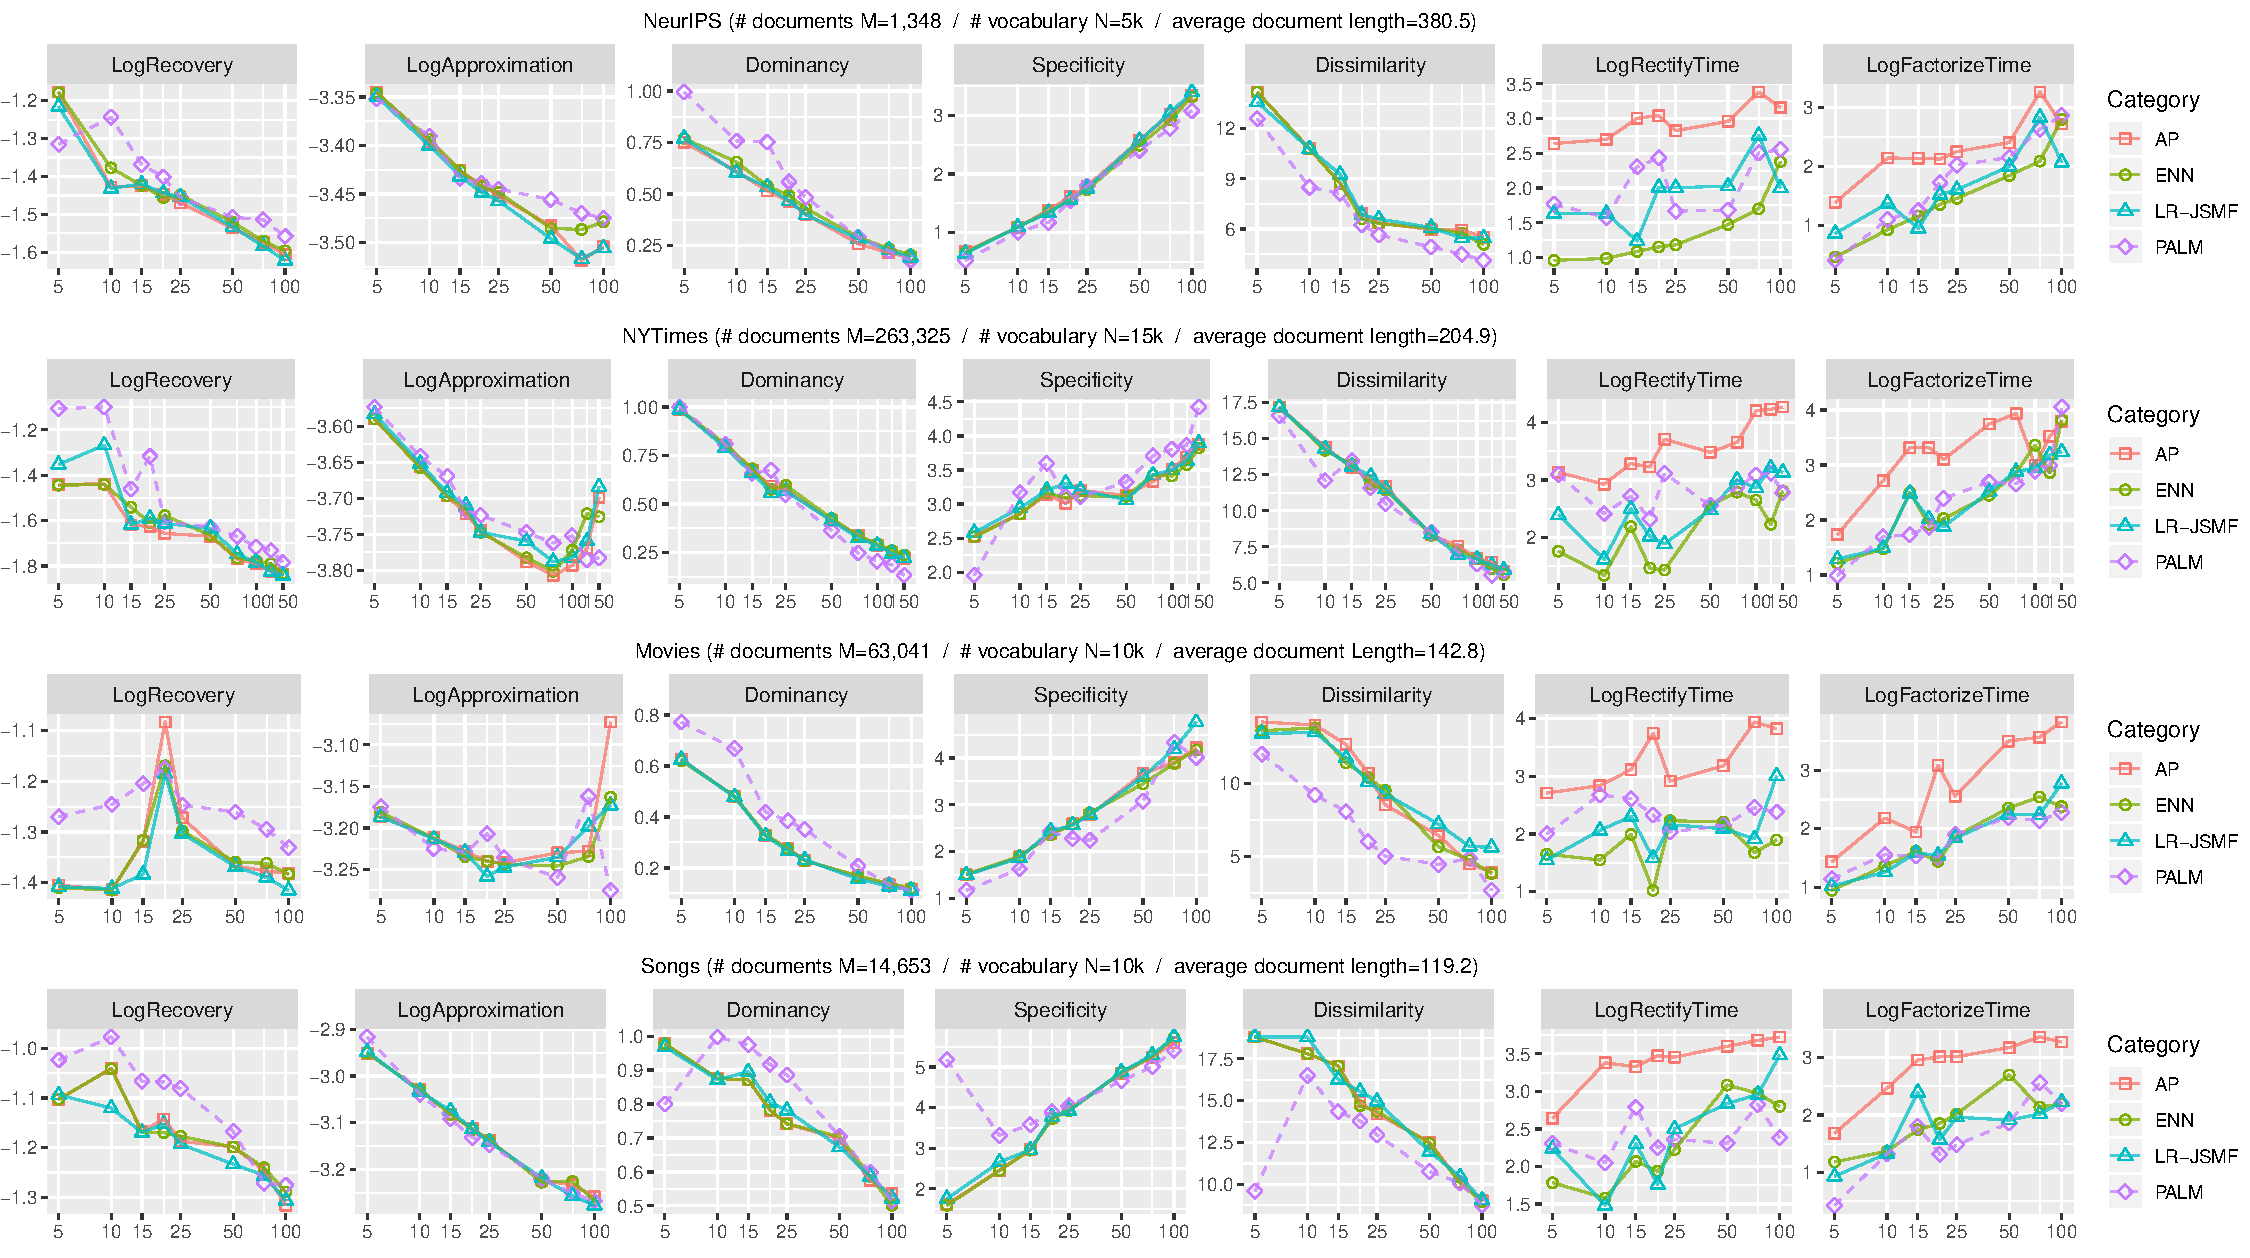
\includegraphics[width=0.97\textwidth, trim={1.0cm 1.0cm 1.0cm 0.0cm}]
	{./ch4/pics/real_MethodsPerTopics_new-plain.pdf}
	\caption{Experiment on four datasets. ENN and LR-JSMF mostly agree with AP,
	whereas PALM has slight inconsistency. The general information of each dataset
	is above the corresponding row. Recovery, approximation, and runtimes are in
	$\log_{10}$ scale. Note that ENN and LR-JSMF are almost two orders of
	magnitude faster than AP. The $x$-axis indicates the number of clusters $K$.
	Lower numbers in $y$-axis are better except Specificity and Dissimilarity.} 
	\label{fig:results-topics}
\end{figure}

A good factorization should be accurate, meaningful, and fast.
In two series of experiments, we show that LR-JSMF maintains model quality while
running in a fraction of the space and time needed for the original JSMF method.
Previous methods have required truncation of the vocabulary even to run on
consumer-grade computers. We show not only that we are able to handle
increasingly large vocabularies without loss of speed, but that using larger
vocabularies measurably improves model quality relative to truncated vocabularies.

For the first series of experiments, we measure the accuracy of each
rectification component as well as the entire pipeline of LR-JSMF. To produce a
strong baseline, we begin with constructing the full co-occurrence $\BC$ from
each of our datasets $\BH$ by \eqref{eqn:unbiased}, and produce the rectified
$\BC_{AP}$ by running Alternating Projection (AP) on $\BC$. Next we compress
$\BC$ into $\BY_{ENN}$ and $\BY_{PALM}$ by running ENN (50 iterations, $|I|\Eq
10K \Plus 1000$) and PALM (100 iterations, $s\Eq1e^{-4}$). For testing our
complete low-rank pipeline, we also construct $(\BV, \BD)$ directly from the raw
data $\BH$ by the randomized eigen-decomposition in Algorithm \ref{alg:lr-jsmf},
learning the compressed statistics \smash{$\BY_{LR-JSMF}$} again by running ENN
initialized with \smash{$\BV \sqrt{\BD}$}. Then we run the Anchor Word algorithm
(AW) on $\BC_{AP}$ and the Low-rank Anchor Word algorithm (LAW) on each of $\BY_
{ENN}$, $\BY_{PALM}$, and $\BY_{LR-JSMF}$.

The goal of rectification is to apply spectral inference to data that does not
follow our modeling assumptions, so we evaluate on real data. In addition to two
standard datasets from the UCI Machine Learning repository (NeurIPS papers and
New York Times articles), we also use two non-textual datasets (Movies and
Songs) previously used to demonstrate the performance of full algorithm with
AP-rectification in \cite{moontae2015nips}. Although our ultimate goal is to
extend JSMF to large vocabularies, we use the same restricted vocabulary as 
\cite{moontae2015nips} for a fair comparison in the first series of experiment.

Figure \ref{fig:results-topics} shows the overall performance of the learned
topic clusters from these four datasets with increasing number of clusters $K$.
Low \textbf{Recovery} error $\frac{1}{N}\sum_i\|\BCbar_{i\ast} - \BBreve_{i\ast}
\BCbar_{S\ast}\|_2$ implies that the learned anchor objects successfully
reconstruct the co\hyp{}occurrence space of the entire objects. Low 
\textbf{Approximation} error $\|\BC-\BB\BA\BB^T\|_2$ means that our
factorization captures most of information given in the unbiased co
\hyp{}occurrence statistics. In real data, low \textbf{Dominancy} $\frac{1}
{K}\sum_k \BA_{kk}$ implies that our models learn more correlations between
clusters. High \textbf{Specificity} \smash{$\frac{1}{K} \sum_k \text{KL}(\BB_
{\ast k}||\sum_i\BC_{\ast i})$} indicates that the learned clusters are
different enough from the corpus distribution, whereas high 
\textbf{Dissimilarity} counts the average number of objects in each cluster that
do not occur among top $20$ in other clusters, showing the interpretable
difference across the learned clusters. We do not report the Cluster Coherence
because it often measures deceptively \cite{chang2009reading}. The first five
columns show that ENN and LR\hyp{}JSMF learn approximately same clusters as JSMF
with the full AP, showing no visible loss in accuracy across all settings. More
importantly, the randomness we introduced into LR\hyp{}JSMF results in a very
low variance over a number of runs. This is important as the stability of
spectral inference is a major advantage relative to MCMC or Variational
Inference. Although PALM deviates a small amount from the other three methods in
a few cases, it mostly achieves the same level of accuracy and follows the
overall trend closely. In terms of runtimes, all of our methods have clear
advantage over AP, gaining $1\sim2$ orders of magnitude speedup in most
situations. Even for applications on relatively small vocabulary sizes, our
algorithms shows a notable improvement in efficiency.

\begin{figure}[ht]
 	\centering
	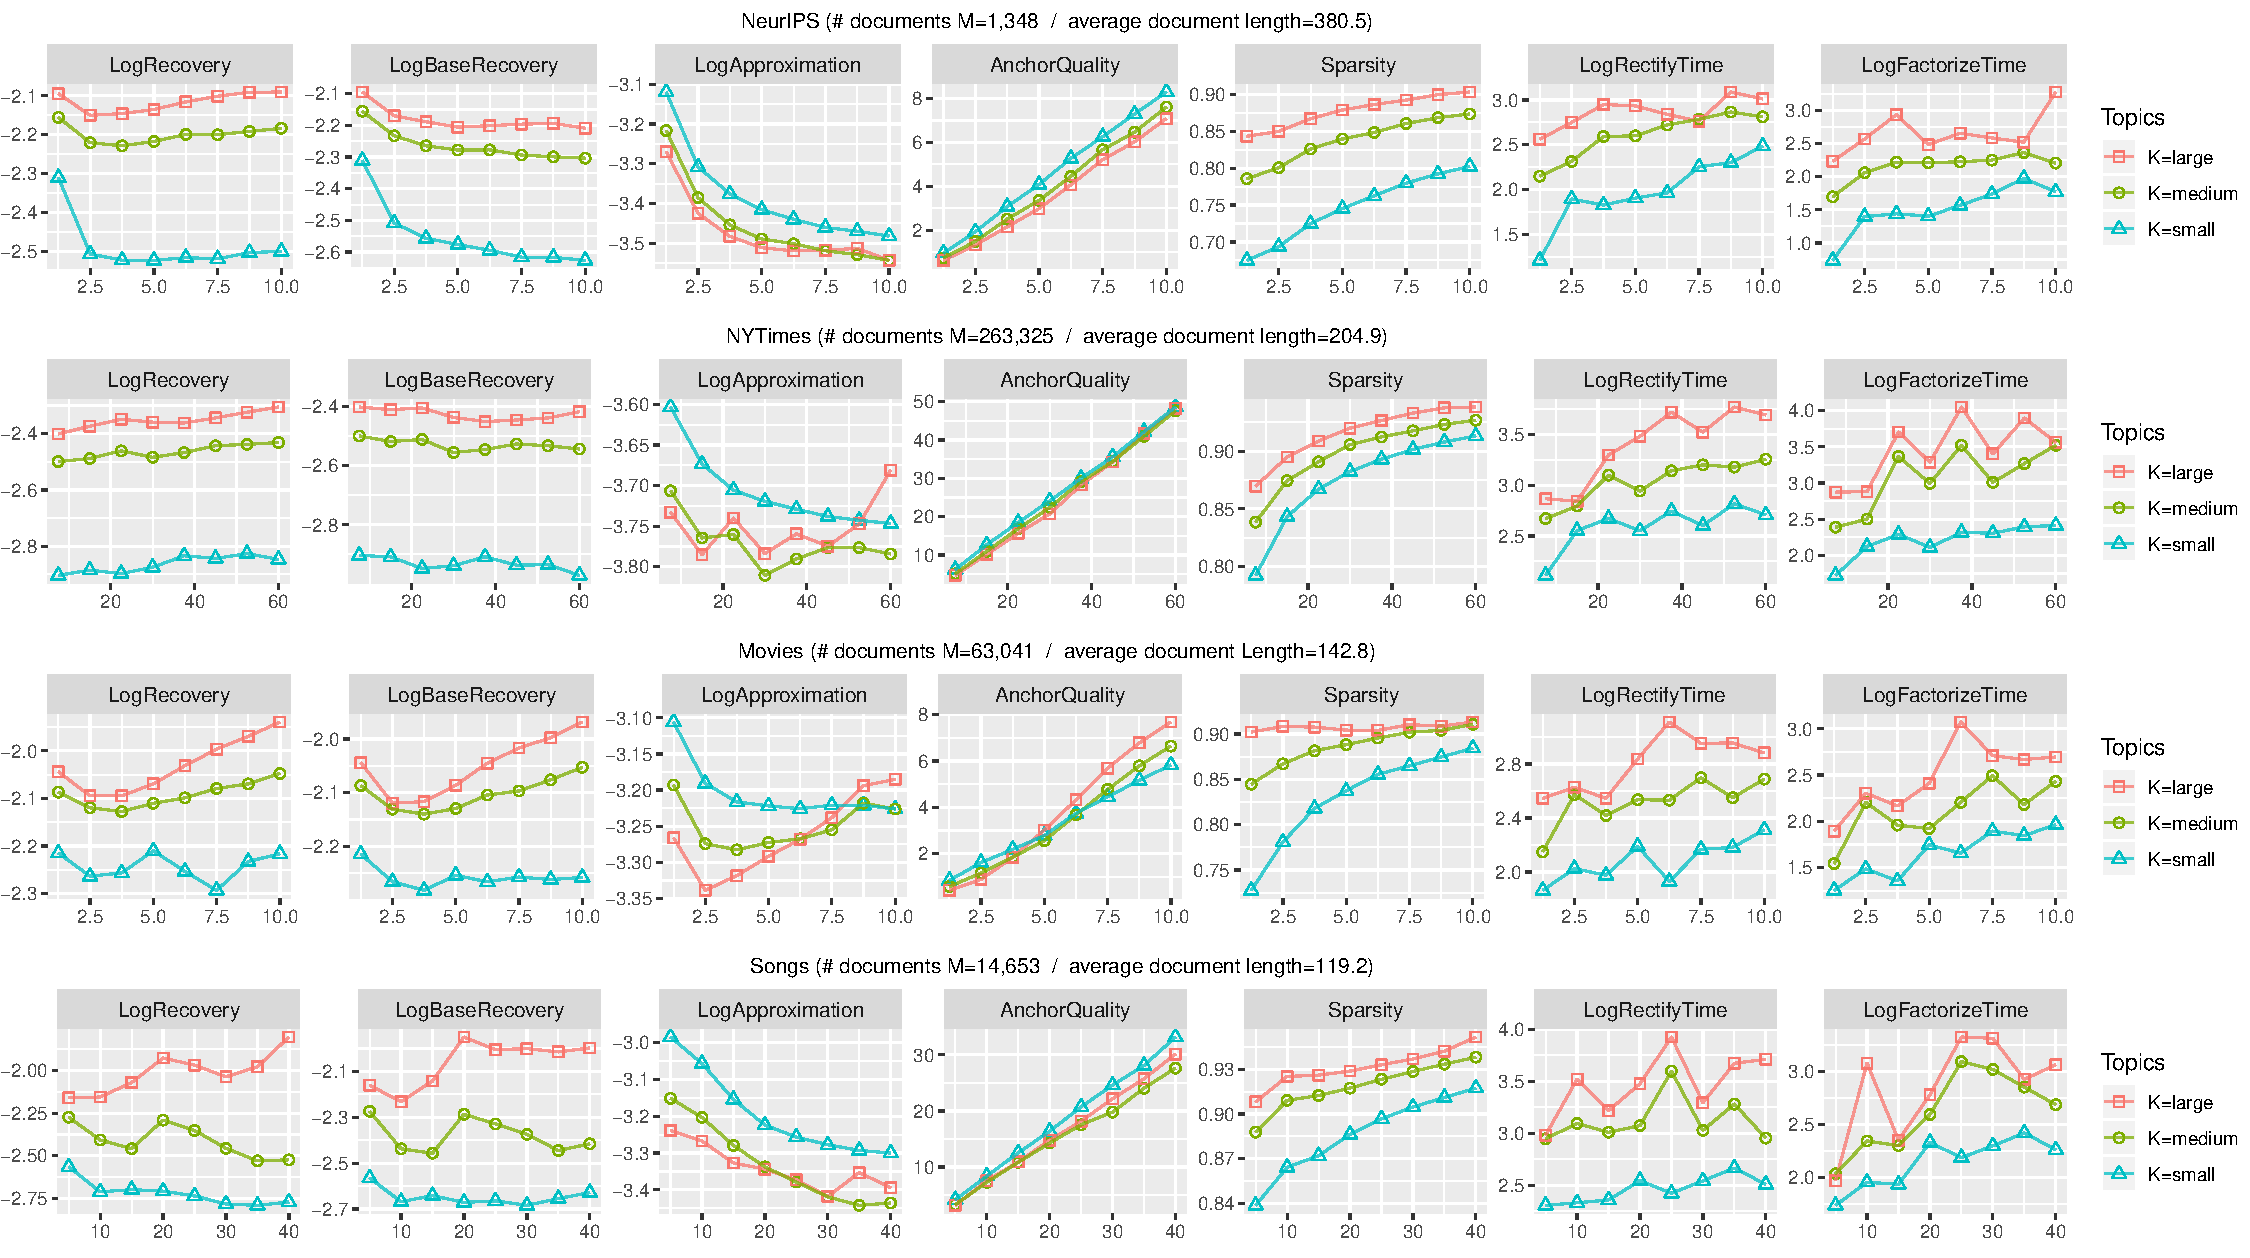
\includegraphics[width=0.97\textwidth, trim={1.0cm 1.0cm 1.0cm 0.0cm}]
	{./ch4/pics/real_TopicsPerVocabs_new-plain.pdf}
	\caption{As we increase the vocabulary size for four collections, anchor
	quality and sparsity improve, but running time is stable. The $x$-axis
	indicates the vocabulary size $N$ in thousands. Values above 15k will not fit
	in memory on standard hardware with previous algorithms.}
	\label{fig:results-vocabs}
\end{figure}

For the second series of experiments, 
we create eight corpora $\{\BH_N, \BH_{2N}, ..., \BH_{8N}\}$ for each dataset
$\BH$ by tailoring their vocabulary sizes as multiples of a base vocabulary of
$N$ objects. In this case we are not able to compare LR-JSMF to previous methods
because we cannot store the full co\hyp{}occurrence matrices for the larger
vocabulary: these models would be impossible. Figure \ref{fig:results-vocabs}
illustrates the overall performance of the learned small/medium/large size
clusters with increasing vocabulary size $N$. Low \textbf{BaseRecovery} means
that the anchor objects from the models with larger vocabulary better
reconstruct the objects in our base vocabulary ($\BH_N$). High  
\textbf{AnchorQuality} indicates that the average rank of the anchor objects
$s_k$ in every other topic clusters than $k$ is high, implying the anchor
objects rarely contribute to other clusters than their own. High 
\textbf{Sparsity} \smash{$(\frac{1}{K} \sum_k \frac{\sqrt{N} - (\|\Bb_k\|_1 /
\|\Bb_k\|_2)}{\sqrt{N} - 1})$} \cite{Hoyer2004} says that our topic clusters are more concentrated on specific objects.

We observe the quality of anchors increases with increasing vocabulary size,
verifying that using larger vocabularies helps better satisfy the separability
assumption. We also verify that a large vocabulary often better approximates the
co\hyp{}occurrence statistics and better reconstructs the co\hyp{}occurrence
space of the \textit{base} vocabulary, but these patterns are not always
consistent in non-textual datasets. In contrast, Sparsity consistently improves,
increasing the interpretability of the learned clusters. Most excitingly, the
running times of ENN and LAW show the scalability of our new rectification and
low-rank algorithm, thereby demonstrating that LR-JSMF is an efficient and
robust pipeline.

Finally, we have also inspected the qualitative behavior of the recovered
clusters, as we increase the vocabulary size. The topic clusters become
significantly more specific, while the clustering of objects is more
conspicuous. Figure \ref{fig:top_words} shows how using a larger vocabulary size
can lead to more distinguishable topics, especially as it allows us to make use
of words that are relatively rare, but used in much narrower contexts. Going
from left to right, we can observe that the set of topic words become more and
more specific: for instance, the topic corresponding to the third row is
slightly vague when observing just the left half of the row, while as we
increase the vocabulary size beyond 5000, we gain access to highly
topic-specific words such as hjb (Hamilton-Jacobi-Bellman equation) or pid 
(Proportional Integral Derivative), which signifies the row's pertinence to
dynamical and control systems. The flip side of the figure shows that words we
would normally consider as non-topical can often be assigned high contributions
towards certain topics. The strong red shade on the bottom left indicates that
words such as ``equivalent'' or ``cambridge'' are strongly connected to the
machine learning literature.

\begin{figure}[ht]
 	\centering
	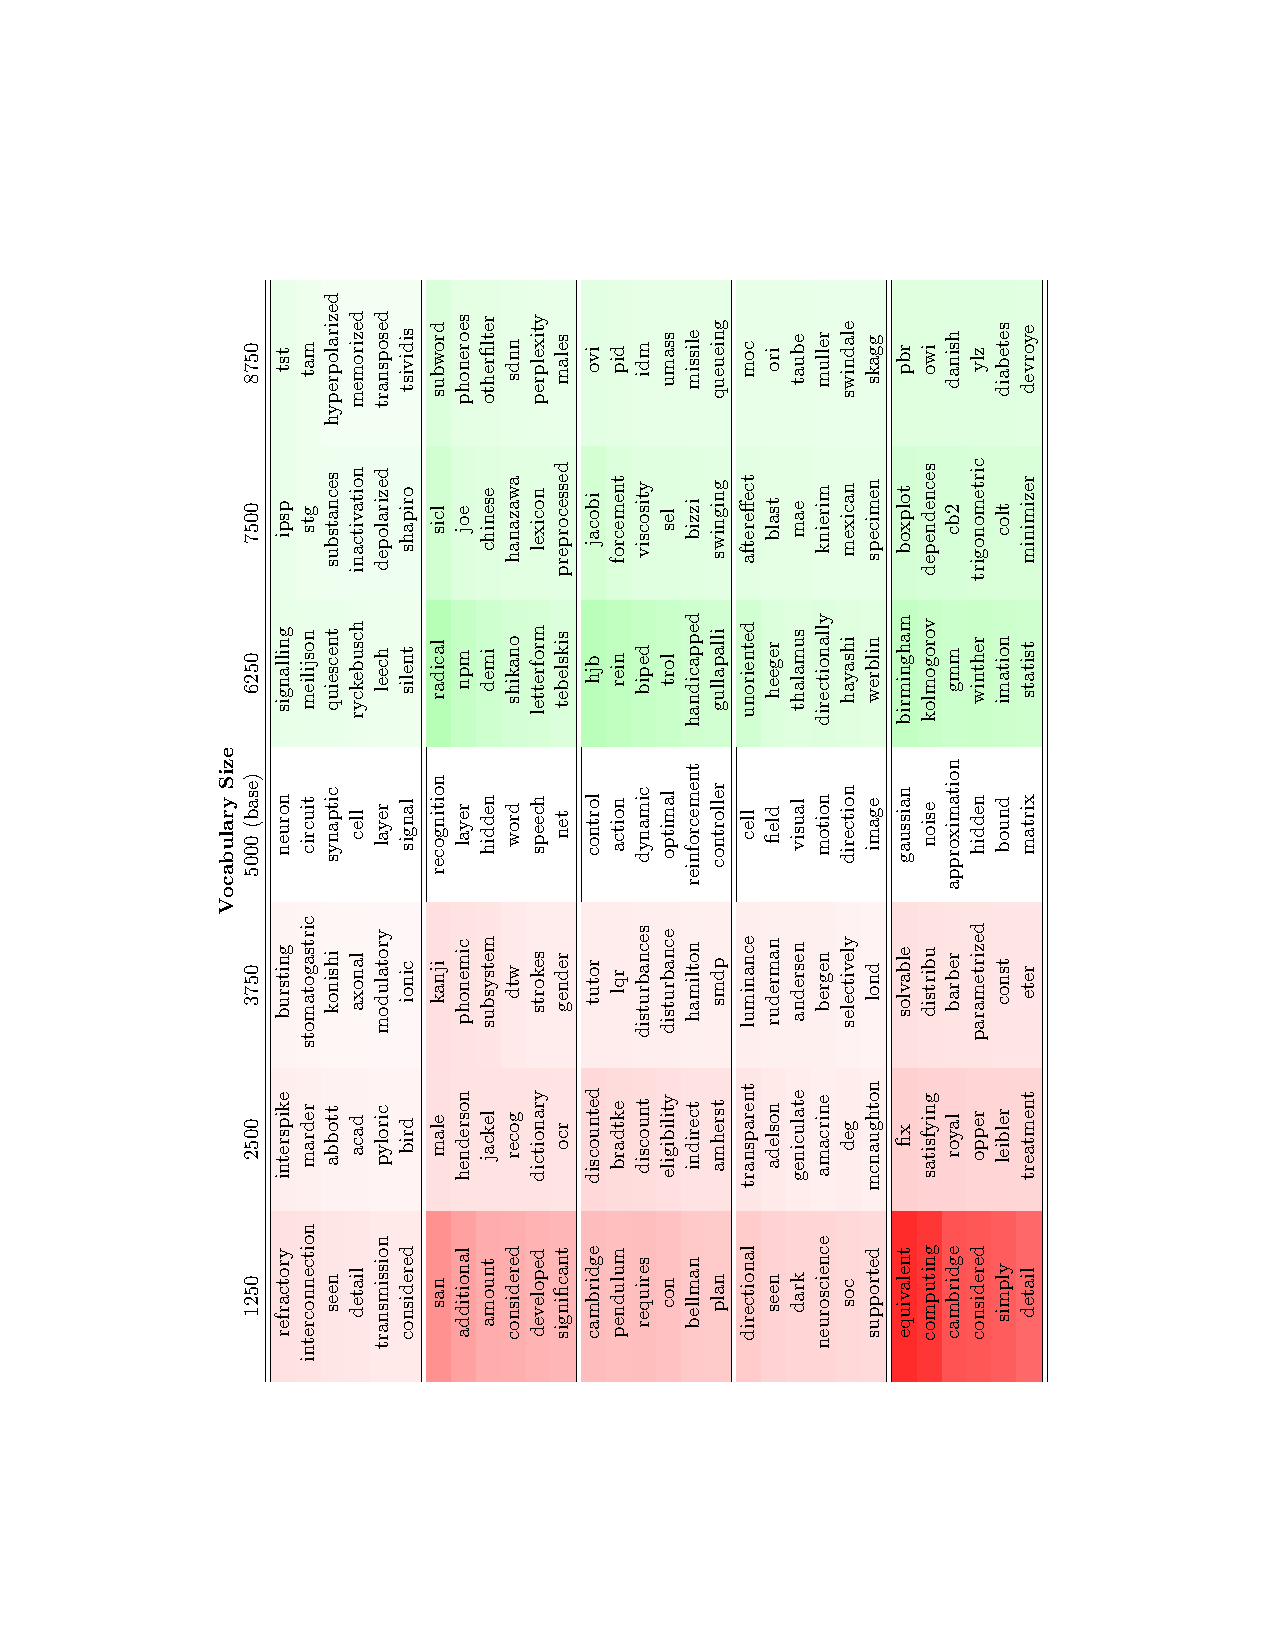
\includegraphics[angle=270, width=1.0\textwidth, trim={2.0cm, 4.5cm, 2.0cm,
	4.5cm}]{./ch4/pics/topWordsFull.pdf}
	\vspace*{-40px}
	\caption{Losses or gains in topic words depending on the vocabulary size. Each
	row represents a topic from the NeurIPS dataset, with the top 6 topical words
	shown in the middle column. The red and green cells denote topic words that
	are lost or gained by shifting the vocabulary size from the default size 5000,
	respectively. The intensities of the colors indicate the words' contributions
	towards the specific topic.} 
	\label{fig:top_words}		
\end{figure}
\FloatBarrier

\section{Conclusion}\label{c4sec:con}
Spectral algorithms provide an appealing alternative for identifying
interpretable low-rank subspaces by simple factorizations of higher-order
moments. But this simplicity is also a weakness: violations of modeling
assumptions destroy performance unless they are handled through rectification,
and the size of the moment matrices limits us to small vocabularies. In this
paper, we developed an efficient and scalable framework: Low-Rank Joint
Stochastic Matrix Factorization. We provide theoretical advances in compressed
matrix factorization, leading to high-quality low-rank non-negative
approximations without quadratic blowup. The method provides orders of magnitude
speedups for rectification even on small vocabularies. Perhaps most importantly,
we can now apply reliable, high-quality factorizations of high-dimensional data
sets on laptop-grade hardware, massively increasing the applicability and
potential use of these algorithms.

\chapter{Weighted K-Means for Electronic Structure Calculation}
	\label{ch5}
	\section{Abstract}\label{c5sec:abs}
	The recently developed interpolative separable density fitting (ISDF)
decomposition is a powerful way for compressing the redundant information in the
set of orbital pairs, and has been used to accelerate quantum chemistry
calculations in a number of contexts. The key ingredient of the ISDF
decomposition is to select a set of non-uniform grid points, so that the values
of the orbital pairs evaluated at such grid points can be used to accurately
interpolate those evaluated at all grid points. The set of non-uniform grid
points, called the interpolation points, can be automatically selected by a QR
factorization with column pivoting (QRCP) procedure. This is the computationally
most expensive step in the construction of the ISDF decomposition. In this work,
we propose a new approach to find the interpolation points based on the
centroidal Voronoi tessellation (CVT) method, which offers a much less expensive
alternative to the QRCP procedure when ISDF is used in the context of hybrid
functional electronic structure calculations. The CVT method only uses
information from the electron density, and can be efficiently implemented using
a K-Means algorithm. We find that this new method achieves comparable accuracy
to the ISDF-QRCP method, at a cost that is negligible in the overall hybrid
functional calculations. For instance, for a system containing $1000$ silicon
atoms simulated using the HSE06 hybrid functional on $2000$ computational cores,
the cost of QRCP-based method for finding the interpolation points costs
$38.1\Sec$, while the CVT procedure only takes $0.7\Sec$.  We also find that the
ISDF-CVT method also enhances the smoothness of the potential energy surface in
the context of \emph{ab initio} molecular dynamics (AIMD) simulations with
hybrid functionals.

\section{Introduction}\label{c5sec:int}
	Orbital pairs of the form $\{\varphi_{i}(\Br)\psi_{j}(\Br)\}_{i,j=1}^{N}$, where
$\varphi_{i}, \psi_{j}$ are single particle orbitals, appear ubiquitously in
quantum chemistry. A few examples include the Fock exchange operator, the MP2
amplitude, and the polarizability operator \cite{SzaboOstlund1989,Martin2004}.
When $N$ is proportional to the number of electrons $N_{e}$ in the system, the
total number of orbital pairs is $N^2\Sim\calO(N_{e}^2)$. On the other
hand, the number of degrees of freedom needed to resolve all orbital pairs on a
dense grid is only $\calO(N_{e})$.  Hence as $N_{e}$ becomes large, the set of
all orbital pairs contains apparent redundant information. In order to compress
the redundant information and to design more efficient numerical algorithms,
many algorithms in the past few decades have been developed. Pseudospectral
decomposition \cite{MurphyJCP1995,ReynoldsJCP1996}, Cholesky decomposition 
\cite{BeebeLinderberg1977,KochSanchezdePedersen2003,AquilantePedersenLindh2007,
ManzerHornMardirossianEtAl2015}, density fitting (DF) or resolution of identity
(RI) \cite{NJP_14_053020_2012,Weigend2002}, and tensor hypercontraction (THC) 
\cite{ParrishHohensteinMartinezEtAl2012,ParrishHohensteinMartinezEtAl2013} are
only a few examples towards this goal. When the single particle orbitals
$\varphi_{i},\psi_{j}$ are already localized functions, ``local methods'' or
``linear scaling methods'' \cite{Goedecker1999, RPP_75_036503_2010_ON,
GuidonHutterVandevondele2010, CP_356_98_2009} can be applied to construct such
decomposition with cost that scales linearly with respect to $N_{e}$. Otherwise,
the storage cost of the matrix to represent all orbital pairs on a grid is
already $\calO(N_{e}^3)$, and the computational cost of compressing the orbital
pairs is then typically $\calO(N_{e}^{4})$.

Recently, Lu and Ying developed a new decomposition called the interpolative
separable density fitting (ISDF) \cite{JCP_302_329_2015_ISDF}, which takes the
following form
\begin{equation}\label{eqn:isdfformat}
  \varphi_{i}(\Br)  \psi_{j}(\Br)\approx \sum_{\mu=1}^{N_{\mu}}
  \zeta_{\mu}(\Br) \left(\varphi_{i}(\Brhat_\mu)\psi_{j}(\Brhat_\mu)\right).
\end{equation}
For a given $\Br$, if we view $[\psi_{i}(\Br)\psi_{j}(\Br)]$ as a row
of the matrix $\{\psi_{i}\psi_{j}\}$ discretized on a dense grid, then the ISDF
decomposition states that all such matrix rows can be approximately expanded
using a linear combination of matrix rows with respect to a selected set of 
\textit{interpolation points} $\{\Brhat_\mu\}_{\mu=1}^{N_{\mu}}$.  The
coefficients of such linear combination, or \textit{interpolating vectors}, are
denoted by $\{\Bzeta_{\mu}(\Br)\}_{\mu=1}^{N_{\mu}}$. Here $N_{\mu}$ can be
interpreted as the numerical rank of the ISDF decomposition. Compared to the
standard density fitting method, the three-tensor $\left\{\varphi_{i}
(\Brhat_\mu)\psi_{j}(\Brhat_\mu)\right\}$ with three indices $i, j, \mu$ takes a
separable form. This reduces the storage cost of the decomposed tensor from
$\calO(N_{e}^3)$ to $\calO(N_{e}^2)$, and the computational cost from $\calO(N_
{e}^{4})$ to $\calO(N_{e}^3)$. Note that if the interpolation points $
\{\Brhat_\mu\}_{\mu=1}^{N_{\mu}}$ are chosen to be on a uniform grid, then the ISDF decomposition reduces to the pseudospectral decomposition, where $N_
{\mu}\Sim\calO(N_{e})$ but with a large preconstant. For instance, the
pseudospectral decomposition can be highly inefficient for molecular systems,
where the grid points in the vacuum contribute nearly negligibly to the orbital
pairs. On the other hand, by selecting the interpolation points carefully, e.g.
through a randomized QR factorization with column pivoting (QRCP) procedure 
\cite{GolubVan2013}, the number of interpolation points can be significantly
reduced. The QRCP based ISDF decomposition has been applied to accelerate a
number of applications, at least in the context of pseudopotential approximation
where the wavefunctions are smooth, including two-electron integral computation 
\cite{JCP_302_329_2015_ISDF}, correlation energy in the random phase
approximation \cite{LuThicke2017}, density functional perturbation theory 
\cite{LinXuYing2017}, and hybrid density functional calculations 
\cite{JCTC_2017_ISDF}. For example, when iterative solvers are used for hybrid
density functional calculations, the Fock exchange operator $V_{X}$ defined in
terms of a set of orbitals $\{\varphi_i\}$ needs to be repeatedly applied to
another set of Kohn-Sham orbitals $\{\varphi_j\}$
\begin{equation}\label{eqn:applyVX}
  \left(V_{X}[\{\varphi_{i}\}]\psi_{j}\right)(\Br) =
  -\sum_{i=1}^{N_{e}} \varphi_{i}(\Br) \int K(\Br,\Br')
  \varphi_{i}(\Br')\psi_{j}(\Br') d\Br'.
\end{equation}
where $K(\Br,\Br')$ is the kernel for the Coulomb or the screened Coulomb
operator.  The integration in Eq. \ref{eqn:applyVX} is often carried out by
solving Poisson-like equations, using e.g. a fast Fourier transform (FFT)
method, and the computational cost is $\calO(N_e^3)$ with a large preconstant.
This is typically the most time consuming component in hybrid functional
calculations, and can be accelerated by the ISDF decomposition for the orbital
pairs $\{\varphi_{i}\psi_{j}\}$.

In Ref.~\cite{JCP_302_329_2015_ISDF}, the interpolation points and the
interpolation vectors are determined simultaneously through randomized QRCP
applied to $\{\psi_{i}(\Br)\psi_{j}(\Br)\}$ directly. We recently found that the
randomized QRCP procedure has $\calO(N_{e}^3)$ complexity but with a relatively
large preconstant, and may not be competitive enough when used repeatedly. In
order to overcome such difficulty, we proposed a different approach in Ref.
~\cite{JCTC_2017_ISDF} that determines the two parts separately and reduces the
computational cost. We use the relatively expensive randomized QRCP procedure to
find the interpolation points in advance, and only recompute the interpolation
vectors whenever $\{\psi_{i}(\Br)\psi_{j}(\Br)\}$ has been updated using an
efficient least squares procedure that exploits the separable nature of the
matrix to be approximated. As a result, we can significantly accelerate hybrid
functional calculations using the ISDF decomposition in all but the first SCF
iteration.

In this work, we further remove the need of performing the QRCP decomposition
completely and, hence, significantly reduce the computational cost. Note that an
effective choice of the set of interpolation points should satisfy the following
two conditions. (1) The distribution of the interpolation points should roughly
follow the distribution of the electron density. In particular, there should be
more points when the electron density is high, and less or even zero points if
the electron density is very low. (2) The interpolation points should not be very
close to each other.  Otherwise, matrix rows represented by the interpolation
points are nearly linearly dependent, and the matrix formed by the interpolation
vectors will be highly ill-conditioned.  The QRCP procedure satisfies both (1)
and (2) simultaneously, and thus is an effective way for selecting the
interpolation points.  Here we demonstrate that (1) and (2) can also be satisfied
through a much simpler centroidal Voronoi tessellation (CVT) procedure applied
to a weight vector such as the electron density.

The Voronoi tessellation technique has been widely used in computer science
\cite{aurenhammer1991voronoi}, and scientific and engineering applications such
as image processing\cite{du2006centroidal}, pattern recognition 
\cite{ogniewicz1995hierarchic}, and numerical integration 
\cite{becke1988multicenter}. The concept of Voronoi tessellation can be simply
understood as follows. Given a discrete set of weighted points, the CVT
procedure divides a domain  into a number of regions, each consisting of a
collection of points that are closest to its weighted centroid. Here we choose
the electron density as the weight, and the centroids as the interpolation
points. The centroids must be located where the electron density is significant,
and hence satisfy the requirement (1). The centroids are also mutually separated
from each other by a finite distance due to the nearest neighbor principle, and
hence satisfy the requirement (2). Although detailed analysis of the error
stemming from such a choice of interpolation points is very difficult for
general nonlinear functions, we find that the CVT procedure approximately
minimizes the residual of the ISDF decomposition in Eq.~\ref{eqn:isdfformat}.
In practice, the CVT procedure only applies to one vector (the electron density)
instead of $\calO(N_{e}^2)$ vectors and hence is very efficient.

We apply the ISDF-CVT method to accelerate hybrid functional calculations in a
planewave basis set. We perform such calculations for different systems with
insulating (liquid water), semiconducting (bulk silicon), and metallic 
(disordered silicon aluminum alloy) characters, as well as ab initio molecular
dynamics (AIMD) simulations. We find that the ISDF-CVT method achieves similar
accuracy to that obtained from the ISDF-QRCP method, with significantly improved
efficiency. For instance, for a bulk silicon system containing $1000$ silicon
atoms computed on $2000$ computational cores with kinetic energy cutoff being
$10\Ha$, the QRCP procedure finds the interpolation points with $38.1\Sec$,
while the CVT procedure only takes $0.7\Sec$. Since the solution of the CVT
procedure is continuous with respect to changes in the electron density, we also
find that the CVT procedure produces a smoother potential energy surface than
that by the QRCP procedure in the context of AIMD simulations.

The remainder of the paper is organized as follows. We briefly introduce the
ISDF decomposition in \S \ref{c5sec:bac}. In \S \ref{c5sec:met} we describe the
ISDF-CVT procedure and its implementation for hybrid functional calculations. We
present numerical results of the ISDF-CVT method in \S 
\ref{c5sec:num}, and conclude in \S \ref{c5sec:con}.

\section{Interpolative Separable Density Fitting (ISDF) decomposition}
	\label{c5sec:bac}
	In this section, we briefly introduce the ISDF decomposition 
\cite{JCP_302_329_2015_ISDF} evaluated using the method developed in Ref. 
\cite{JCTC_2017_ISDF}, which employs a separate treatment of the interpolation
points and interpolation vectors.

First, assume the interpolation points $
\{\Brhat_\mu\}_{\mu=1}^{N_{\mu}}$ are known, then the interpolation vectors can
be efficiently evaluated using a least squares method as follows. Using a linear
algebra notation, Eq. \ref{eqn:isdfformat} can be written as
\begin{equation}\label{eqn:isdflineq}
  \BZ \approx \BTheta \BC,
\end{equation}
where each column of $\BZ$ is given by $\BZ_{ij}(\Br)=\varphi_{i}(\Br)\psi_{j}
(\Br)$ sampled on a dense real space grids $\{\Br_{i}\}_{i=1}^{N_g}$, and
$\BTheta = [\Bzeta_1, \Bzeta_2, ..., \Bzeta_{N_{\mu}}]$ contains the
interpolating vectors. Each column of $\BC$ indexed by $(i,j)$ is given by
\begin{equation}
\left[ \varphi_{i}(\Brhat_1)\psi_{j}(\Brhat_1),\; \cdots,\;
    \varphi_{i}(\Brhat_\mu)\psi_{j}(\Brhat_\mu),\; \cdots,\;
    \varphi_{i}(\Brhat_{N_{\mu}})\psi_{j}(\Brhat_{N_{\mu}})\right]^T.
\end{equation}
Eq. \ref{eqn:isdflineq} is an overdetermined linear system with respect to the
interpolation vectors $\BTheta$. The least squares approximation to the solution
is given by
\begin{equation}\label{eq:Theta}
  \BTheta = \BZ\BC^T (\BC\BC^T)^{-1}.
\end{equation}
It may appear that the matrix-matrix multiplications $\BZ\BC^T$ and $\BC\BC^T$
take $\calO(N_{e}^{4})$ operations because the size of $\BZ$ is $N_g \times N^2$
and the size of $\BC$ is $N_{\mu} \times N^2$.  However, both multiplications
can be carried out with fewer operations due to the separable structure of $\BZ$
and $\BC$. The computational complexity for computing the interpolation vectors
is $\calO(N_{e}^{3})$, and numerical results indicate that the preconstant is
also much smaller than that involved in hybrid functional calculations 
\cite{JCTC_2017_ISDF}. Hence the interpolation vectors can be obtained
efficiently using the least squares procedure.

The problem for finding a suitable set of interpolation points $\{\Brhat_\mu\}_
{\mu=1}^{N_{\mu}}$ can be formulated as the following linear algebra problem.
Consider the discretized matrix $\BZ$ of size $N_{g}\times N^2$, and find $N_
{\mu}$ rows of $\BZ$ so that the rest of the rows of $\BZ$ can be approximated
by the linear combination of the selected $N_{\mu}$ rows. This is called an
interpolative decomposition \cite{SIAM_13_727_1992_QRCP}, and a standard method
to achieve such a decomposition is the QR factorization with column pivoting 
(QRCP) procedure \cite{SIAM_13_727_1992_QRCP} as
\begin{equation}\label{eqn:QRCP}
  \BZ^{T} \BPi = \BQ\BR.
\end{equation}
Here $\BZ^T$ is the transpose of $\BZ$, $\BQ$ is an $N^2 \times N_g$ matrix that
has orthonormal columns, $\BR$ is an upper triangular matrix, and $\BPi$ is a
permutation matrix chosen so that the magnitude of the diagonal elements of
$\BR$ form an non-increasing sequence.  The magnitude of each diagonal element
$\BR$ indicates how important the corresponding column of the permuted $\BZ^T$
is, and whether the corresponding grid point should be chosen as an
interpolation point. The QRCP factorization can be terminated when the $(N_
{\mu}+1)$-th diagonal element of $\BR$ becomes less than a predetermined
threshold. The leading $N_{\mu}$ columns of the permuted $\BZ^T$ are considered
to be linearly independent numerically. The corresponding grid points are chosen
as the interpolation points. The indices for the chosen interpolation points $
\{\Brhat_\mu\}$ can be obtained from indices of the nonzero entries of the first
$N_{\mu}$ columns of the permutation matrix $\BPi$.

The QRCP decomposition satisfies the requirements (1) and (2) discussed in \S
\ref{c5sec:int}. First, QRCP permutes matrix columns of $\BZ^{T}$ with large
norms to the front, and pushes matrix columns of $\BZ^{T}$ with small norms to
the back. Note that the square of the vector 2\hyp{}norm of the column of $\BZ^
{T}$ labeled by $\Br$ is just
\begin{equation}\label{eqn:Znorm}
  \sum_{i,j=1}^{N} \varphi_{i}^2(\Br) \varphi_{j}^2(\Br) =
  \left(\sum_{i=1}^{N} \varphi_{i}^2(\Br)\right) \left(\sum_{j=1}^{N}
  \psi_{j}^2(\Br)\right).
\end{equation}
In the case when $\varphi_{i},\psi_{j}$ are the set of occupied orbitals, the
norm of each column of $\BZ^{T}$ is simply the electron density. Hence the
interpolation points chosen by QRCP will occur where the electron density is
significant. Second, once a column is selected, all other columns are
immediately orthogonalized with respect to the chosen column. Hence nearly
linearly dependent matrix columns will not be selected repeatedly. As a result,
the interpolation points chosen by QRCP are well separated spatially.

It turns out that the direct application of the QRCP procedure (Eq. 
\ref{eqn:QRCP}) still requires $\calO(N_{e}^{4})$ computational complexity.  The
key idea used in Ref. \cite{JCP_302_329_2015_ISDF} to lower the cost is to
randomly subsample columns of the matrix $\BZ$ to form a smaller matrix
$\BZtilde$ of size $N_{g}\times \widetilde{N}_\mu$, where $\widetilde{N}_\mu$ is
only slightly larger than $N_{\mu}$.  Applying the QRCP procedure to this
subsampled matrix $\BZtilde$ approximately yields the choice of interpolation
points, but the computational complexity is reduced to $\calO(N_{e}^3)$. In the
context of hybrid density functional calculations, the cost of the randomized
QRCP method can be comparable to that of applying the exchange operator in the
planewave basis set \cite{JCTC_2017_ISDF}. However, the ISDF decomposition can
still significantly reduce the computational cost, since the interpolation
points only need to be performed once for a fixed geometric configuration.

\section{Centroidal Voronoi Tessellation based ISDF decomposition}
	\label{c5sec:met}
	In this section, we demonstrate that the interpolation points can also be
selected from a Voronoi tessellation procedure. For a $d$-dimensional space, the
Voronoi tessellation partitions a set of points $\{\Br_{i}\}_{i=1}^{N_{g}}$ in
$\BBR^{d}$ into a number of disjoint cells. The partition is based on the
distance of each point to a finite set of points, called its generators. In our
context, let $\{\Brhat_\mu\}_{\mu=1}^{N_{\mu}}$ denote such a set of generators,
and the corresponding cell, $\calC_\mu$, of a given generator $\Brhat_\mu$ is
defined as a cluster of points
\begin{equation}\label{eqn:vcell}
  \calC_\mu = \{\Br_{i} ~\vert~\dist(\Br_{i}\,,\, \Brhat_\mu) <
  \dist(\Br_{i}\, ,\, \Brhat_\nu) \textrm{ for all } \nu \neq \mu\}.
\end{equation}
The distance can be chosen to be any metric, e.g. the $L_2$ distance as $\dist
(\Br\,,\,\Br')=\norm{\Br-\Br'}_2$. In the case when the distances of a point
$\Br$ to $\Brhat_\mu, \Brhat_\nu$ are exactly the same, we may arbitrarily
assign $\Br$ to one of the clusters.

The Centroidal Voronoi tessellation (CVT) is a specific type of Voronoi
tessellation in which the generator $\Brhat_\mu$ is chosen to be the centroid of
its cell. Given a weight function $\rho(\Br)$ (such as the electron density),
the centroid of a cluster $\calC_\mu$ is defined as
\begin{equation}\label{eqn:centcomp}
  \Bc(\calC_\mu) = \frac{\sum_{\Br_{j}\In \calC_\mu} \Br_j\;\rho
  (\Br_j)}{\sum_{\Br_j\In \calC_\mu}\rho(\Br_j)}.
\end{equation}
Combined with the $L_2$ distance, CVT can be viewed as a minimization problem
over both all possible partition of the cells and the centroids as \cite{MacQueen1967}
\begin{equation}\label{eqn:CVT}
  \{\calC_\mu^\ast,\Bc_{\mu}^{*}\} = \argmin_{\{\calC_\mu, \Bc_{\mu}\}} \sum_
  {\mu=1}^{N_{\mu}} \sum_{\Br_k\in \calC_\mu}\rho(\Br_k)\norm{\Br_i-\Bc_{\mu}}^2,
\end{equation}
and the interpolation points are then chosen to be the minimizers
$\Brhat_\mu=\Bc_{\mu}(\calC_\mu^\ast)=\Bc_{\mu}^{\ast}$. Following the
discussion in \S \ref{c5sec:int}, the electron density as the weight function~
\eqref{eqn:CVT} enforces that the interpolation points should locate at points
where the electron density is significant and hence satisfies the requirement 
(1). Since the cells $\calC_\mu^\ast$ are disjoint, the centroids $\Bc_{\mu}^
\ast$ are also separated by a finite distance away from each other and hence
satisfies the requirement (2). Because the ISDF decomposition is a highly
nonlinear process, in general we cannot expect the choice of interpolation
points from CVT decomposition to maximally reduce the error of the
decomposition. Instead, we demonstrate that the choice of the interpolation
points from CVT approximately minimizes the residual for the ISDF decomposition,
and hence provides a heuristic solution to the problem of finding interpolation
points.

\begin{theorem}
  When the set of electron orbitals $\{\varphi_i\}$ are Lipschitz continuous,
  CVT method approximately minimizes the residual error of the ISDF
  decomposition.
\end{theorem}
\begin{proof}
  For simplicity we assume the limiting case where $\varphi_{i}=\psi_{i}$, and
  hence each row of $\BZ$ is $\BZ(\Br)=[\varphi_{i}(\Br)\varphi_{j}(\Br)]_
  {i,j=1}^N$.

  Now suppose we cluster all matrix rows of $\BZ$ into sub-collections $
  \{\calC_\mu\}_{\mu=1}^{N_\mu}$, and for each $\calC_\mu$ we choose a
  representative matrix row $\BZ(\Br_\mu)$. Then the error of the ISDF can be
  approximately characterized as
  \begin{equation}\label{eqn:ISDFerror}
    R = \sum_{\mu = 1}^{N_\mu}\sum_{\Br_k\In \calC_\mu}\norm{\BZ(\Br_k)-
    \Proj_{\Span\{\BZ(\Br_{\mu})\}}\BZ(\Br_k)}^2,
  \end{equation}
  where the projection is defined according to the $L_2$ inner product as
  \begin{equation}\label{eqn:Zprojection}
    \Proj_{\Span\{\BZ(\Br_{\mu})\}}\BZ(\Br_k) = \frac{\BZ(\Br_{k})\cdot \BZ
    (\Br_\mu)}{\BZ(\Br_\mu)\cdot \BZ(\Br_\mu)}\BZ(\Br_{\mu}).
  \end{equation}
  Let $\BPhi$ be the $N_{g} \times N$ matrix with each row $\BPhi(\Br) = 
  [\varphi_i(\Br)]_{i=1}^N$, then the electron density $\rho(\Br)$ is equal to
  $\Phi(\Br)\cdot \Phi(\Br)$. Using the relation
  \begin{equation}\label{eqn:ZtoPhi}
    \BZ(\Br_\mu)\cdot \BZ(\Br_\mu) = (\BPhi(\Br_{\mu})\cdot \BPhi(\Br_{\mu}))^2
    = \rho(\Br_{\mu})^2,
  \end{equation}
  we have
  \begin{align}
    R &= \sum_{\mu=1}^{N_\mu}\sum_{\Br_k\In \calC_\mu}\rho(\Br_k)^2 \left(1-
    \frac{(\BPhi(\Br_{k})\cdot\BPhi(\Br_{\mu}))^4}{\rho(\Br_k)^2\rho
    (\Br_\mu)^2}\right)\\
    &= \sum_{\mu=1}^{N_\mu}\sum_{\Br_k\In \calC_\mu}\rho(\Br_k)^2 [1-\cos^4
    (\theta(\Br_k,\Br_\mu))].
  \end{align}
  Here $\theta(\Br_{k},\Br_{\mu})$ is the angle between the vectors $\BPhi(\Br_
  {k})$ and $\BPhi(\Br_{\mu})$. Since
  \begin{align}
    \rho(\Br_k) [1-\cos^4(\theta(\Br_k,\Br_\mu))] &\Leq 2 \BPhi(\Br_{k})\cdot
    \BPhi(\Br_{k})\sin^{2}(\theta(\Br_k,\Br_\mu)) \\
    &\Leq 2 \norm{\BPhi(\Br_{k})-\BPhi(\Br_{\mu})}^2,
  \end{align}
  we have
  \begin{align}
    R &\Leq 2 \sum_{\mu=1}^{N_\mu}\sum_{\Br_k\in \calC_\mu}\rho(\Br_k) 
    \norm{\BPhi(\Br_{k})-\BPhi(\Br_{\mu})}^2 \\
    &\approx 2 \sum_{\mu=1}^{N_\mu}\sum_{\Br_k\in \calC_\mu}\rho(\Br_k)
    \norm{\nabla_{\Br}\BPhi(\Br_{\mu})}^2 \norm{\Br_{k}-\Br_{\mu}}^2.
  \end{align}
  If we bound the gradient of $\BPhi(\Br)$ by its Lipschitz constant, or simply
  neglect the spatial inhomogeneity in the electron orbitals, we arrive at the
  minimization criterion for the centroidal Voronoi tessellation decomposition.
\end{proof}

Many algorithms have been developed to efficiently compute the Voronoi
tessellation \cite{medvedev1986algorithm}. One most widely used method is the
Llyod's algorithm \cite{lloyd1982least}, which in discrete case is equivalent to
the K-Means algorithm \cite{MacQueen1967}. The K-Means algorithm is an iterative
method that greedily minimizes the objective by taking alternating steps between
$\{\calC_\mu\}$ and $\{\Bc_\mu\}$. In this work, we adopt a weighted version of
the K-Means algorithm, which is demonstrated in Algorithm \ref{alg:wkmean}. Note
that the K-Means algorithm can be straightforwardly parallelized. We distribute
the grid points evenly at the beginning. The classification step is the most
time consuming step, and can be locally computed for each group of grid points.
After this step, the weighted sum and total weight of all clusters can be
reduced from and broadcast to all processors for the next iteration.


\begin{algorithm}
  \caption{Weighted K-Means Algorithm to Find Interpolation Points for Density
  Fitting}\label{alg:wkmean}
  \SetKwInOut{Input}{Input}
  \SetKwInOut{Output}{Output}
  \SetKwRepeat{Do}{do}{while}
  \SetKwFor{For}{for}{}{end for}
  \SetKwIF{If}{ElseIf}{Else}{if}{}{else if}{else}{end if}
  \DontPrintSemicolon
  \Input{Grid points $\{\Br_i\}_{i=1}^{N_{g}}$, Weight function $\rho(\Br)$,
  Initial centroids $\{\Bc^{(0)}_\mu\}$}
  \Output{Interpolation points $\{\Brhat_\mu\}_{\mu=1}^{N_{\mu}}$}
  \textbf{Set} $t\gets 0$\;

  \Do{$\{\Bc^{(t)}_\mu\}$ \textrm{\upshape not converged and maximum steps not
  reached}}{
    \textbf{Classification step:}\;
    \For{$i = 1$ \KwTo $N_g$}{
      Assign point $\Br_{i}$ to the cluster $\calC^{(t)}_{\mu}$
      \textbf{if} $\Bc^{(t)}_\mu$ is the closest centroid to $\Br_i$\;
    }
    \;
    \textbf{Update step:}\;
    \For{$\mu = 1$ \KwTo $N_\mu$}{
      $\Bc^{(t+1)}_\mu \gets
      {\sum_{\Br_{j}\In \calC^{(t)}_{\mu}}\Br_j\;\rho(\Br_j)}/{\sum_{\Br_j\In
      \calC^{(t)}_\mu}\rho(\Br_j)}$\;
    }
    \textbf{Set} $t\gets t+1$\;
  }
  \For{$\mu = 1$ \KwTo $N_\mu$}{
    \textbf{Set} $\Brhat_\mu\gets \Bc^{(t)}_{\mu}$\;
  }
\end{algorithm}

In order to demonstrate the CVT procedure, we consider the weight function $\rho
(\Br)$ given by the summation of four Gaussian functions in a 2D domain. The
initial choice of centroids, given by 40 uniformly distributed random points,
together with its associated Voronoi tessellation are plotted in Figure~
\ref{fig:CVT} (a). Figure~\ref{fig:CVT} (b) demonstrates the converged centroids
and the associated Voronoi tessellation using the weighted K-Means algorithm. We
observe that the centroids concentrate on where the weight function is
significant, and are well-separated.

\begin{figure}[htbp]
  \begin{center}
    \includegraphics[width=\textwidth]{./ch5/pics/CVT.pdf}
  \end{center}
  \caption{Schematic illustration of the CVT procedure in a 2D domain, including
  (a) initial random choice of centroids and Voronoi tessellation and centroidal
  Voronoi tessellation generated by the weighted K-Means algorithm. The weight
  function is given by  the linear superposition of 4 Gaussian functions.}
  \label{fig:CVT}
\end{figure}

We also show how the interpolation points are placed and moved in real chemical
systems, i.e. the ammonia-borane (BH$_3$NH$_3$) decomposition reaction process.
Figure~\ref{fig:BH3NH3} (a) shows the electron density of the molecule at the
compressed, equilibrium, and dissociated configurations, respectively, according
to the energy landscape in Fig.~\ref{fig:BH3NH3} (c). We plot the interpolation
points found by the weighted K-Means algorithm in Fig.~\ref{fig:BH3NH3} (b). At
the compressed configuration, all the interpolation points are distributed
evenly around the molecule. As the bond length increases, some interpolation
points are transferred from BH$_3$ to NH$_3$. Finally at the dissociated
configuration, NH$_3$ has more interpolation points around the molecule, since
there are more electrons in NH$_3$ than BH$_3$. Along the decomposition reaction
process, both the transfer of the interpolation points and the potential energy
landscape are smooth with respect to the change of the bond length.


\begin{figure}[htbp]
  \begin{center}
    \includegraphics[width=\textwidth]{./ch5/pics/BH3NH3.pdf}
  \end{center}
  \caption{The decomposition reaction process of BH$_3$NH$_3$ computed with
  hybrid functional (HSE06) calculations by using the CVT procedure to select
  interpolation points, including (a) the electron density (yellow isosurfaces),
  (b) the interpolation points (yellow squares) $\{\Brhat_\mu\}_{\mu=1}^{N_
  {\mu}}$ ($N_{\mu}$ = 8) selected from the real space grid points $\{\Br_{i}\}_
  {i=1}^{N_{g}}$ ($N_{g}$ = 100$^3$ and $E_{\text{cut}}$ = 60 Ha) when the BN
  distance respectively is 1.3, 1.7 and 2.8 {\AA} and (c) the binding energy as
  a function of BN distance for BH$_3$NH$_3$ in a 10 {\AA} $\times$ 10 {\AA}
  $\times$ 10 {\AA} box. The white, pink and blue pink balls denote hydrogen,
  boron and nitrogen atoms, respectively.}
  \label{fig:BH3NH3}
\end{figure}

\section{Numerical results}\label{c5sec:num}
	We demonstrate the accuracy and efficiency of the ISDF-CVT method for hybrid
functional calculations by using the DGDFT (Discontinuous Galerkin Density
Functional Theory) software package \cite{JCP_231_2140_2012_DGDFT,
JCP_143_124110_2015_DGDFT,PCCP_17_31397_2015_DGDFT, JCP_145_154101_2016_DGDFT,
JCP_335_426_2017_DGDFT}. DGDFT is a massively parallel electronic structure
software package designed for large scale DFT calculations involving up to tens
of thousands of atoms. It includes a self-contained module called PWDFT for
performing planewave based electronic structure calculations (mostly for
benchmark and validation purposes). We implemented the ISDF-CVT method in PWDFT.
We use the Message Passing Interface (MPI) to handle data communication. We use
the Hartwigsen-Goedecker-Hutter (HGH) norm-conserving pseudopotential
\cite{PRB_58_3641_1998_HGH}. The atomic valence electron configuration is 1s$^1$
for the H atom, 2s$^2$2p$^1$ for the B atom, 2s$^2$2p$^3$ for the N atom,
2s$^2$2p$^4$ for the O atom, 3s$^2$3p$^2$ for the Si atom in our DFT
calculations, respectively. All calculations use the HSE06 functional 
\cite{JCP_124_219906_2006_HSE06}, carried out on the Edison systems at the
National Energy Research Scientific Computing Center (NERSC). Each node consists
of two Intel ``Ivy Bridge'' processors with 24 cores in total and 64 gigabyte 
(GB) of memory. Our implementation only uses MPI. The number of cores is equal
to the number of MPI ranks used in the simulation.


In this section, we demonstrate the performance of the ISDF-CVT method for
accelerating hybrid functional calculations by using three types of systems 
\cite{JCTC_2017_PCDIIS}. They consist of bulk silicon systems (Si$_{64}$, Si$_
{216}$, and Si$_{1000}$), a bulk water system with $64$ molecules ((H$_2$O)$_
{64}$), and a disordered silicon aluminum alloy system (Al$_{176}$Si$_{24}$).
Bulk silicon systems (Si$_{64}$, Si$_{216}$ and Si$_{1000}$) and bulk water
system ((H$_2$O)$_{64}$) are semiconducting with a relatively large energy gap
$E_\text{gap} > 1.0$ eV, and the Al$_{176}$Si$_{24}$ system is metallic with a
small energy gap $E_\text{gap} < 0.1$ eV. All systems are closed shell systems,
and the number of occupied bands is $N_\text{band} = N_{e}/2$, where $N_e$ is
the number of valence electrons. In order to compute the energy gap in the
systems, we also include two unoccupied bands in all calculations.


\subsection{\numintitle{Accuracy: Si$_{216}$ and Al$_{176}$Si$_{24}$}}
\label{c5subsec:accuracy}

We demonstrate the accuracy of the CVT-based ISDF decomposition in the hybrid
functional calculation for semiconducting Si$_{216}$ and metallic Al$_{176}$Si$_
{24}$ systems, respectively. Although there is no general theoretical guarantee
for the convergence of the K-Means algorithm and the convergence can depend
sensitively on the initialization \cite{arthur2006slow,arthur2007k}, we find
that, in the current context,  initialization to have little impact on the final
accuracy of the approximation. Hence we use random initialization for the
K-Means algorithm. In all calculations, the adaptively compressed exchange (ACE)
technique is used to accelerate hybrid functional calculations without loss of
accuracy \cite{JCTC_12_2242_2016_ACE}. The results obtained in this work are
labeled as ACE-ISDF (CVT), which are compared against those obtained from the
previous work based on the QRCP decomposition \cite{JCTC_2017_ISDF} labeled as
ACE-ISDF (QRCP). In both cases, we introduce a rank parameter $c$ to control the
trade-off between efficiency and accuracy, by setting the number of
interpolation points $N_\mu = cN_e$. We measure the error using the valence band
maximum (VBM) energy level, the conduction band minimum (CBM) energy level, the
energy gap, the Hartree-Fock exchange energy, the total energy, and the atomic
forces, respectively. We remark that, in ISDF-CVT and ISDF-QRCP, the atomic
force is computed directly using the Hellmann-Feynman formula, thereby neglects
the Pulay force contribution from the change of the interpolation points. On the
other hand, there is no Pulay contribution in the ACE formulation, and the
Hellmann-Feynman force $F_I^\text{ACE}$ can be used as the reference solution.

The last three quantities are defined as
\begin{align*}
	\Delta{E_\text{HF}} &= \abs{E_\text{HF}^\text{ACE-ISDF (CVT)} - E_\text{HF}^
	\text{ACE}}/N_{A}\\
	\Delta{E} &= \abs{E^\text{ACE-ISDF (CVT)} - E^\text{ACE}}/N_{A}\\
	{\Delta}F &= \max_I\norm{F_I^\text{ACE-ISDF (CVT)} - F_I^\text{ACE}}
\end{align*}
where $N_A$ is the number of atoms and $I$ is the atom index.

Table~\ref{tab:Accuracy} shows that the accuracy of the ACE-ISDF (CVT) method
can systematically improve as the rank parameter $c$ increases. When the rank
parameter is large enough ($\mathbin{\Geq}20.0$), the results from ACE-ISDF 
(CVT) are fully comparable (the energy error is below $10^{-6}\HaPA$ and the
force error is below $10^{-5}\HaPB$) to those obtained from the benchmark
calculations. Furthermore, for a moderate choice of the rank parameter $c=6.0$,
the error of the energy per atom reaches below the chemical accuracy of 1
kcal/mol ($1.6\times 10^{-3}\HaPA$), and the error of the force is around $10^
{-3}\HaPB$. This is comparable to the accuracy obtained from ACE-ISDF (QRCP),
and to e.g. linear scaling methods for insulating systems with reasonable amount
of truncation needed to achieve significant speedup \cite{JCTC_11_4655_2015}. In
fact, when compared with ACE-ISDF (QRCP) in Figure~\ref{fig:Si216Al176Si24}, we
find that the CVT based ISDF decomposition achieves slightly higher accuracy,
though there is no theoretical guarantee for this to hold in general. The last
column of Table~\ref{tab:Accuracy} shows the runtime of the K-Means algorithm.
As $c$ increases, the number of interpolation points as well as the number of
cells increases proportionally. Hence we observe that the runtime of K-Means
scales linearly with respect to $c$.

\begin{table}[htbp]
	\centering
	\caption{Accuracy of ACE-ISDF Based Hybrid Functional Calculations 
	(HSE06) Obtained by Using the CVT method To Select Interpolation Points,
	with Varying Rank Parameter $c$ for Semiconducting Si$_{216}$ and Metallic
	Al$_{176}$Si$_{24}$ Systems\textsuperscript{$\alpha$}.}\label{tab:Accuracy}
	\begin{threeparttable}
		\begin{tabular}{cccccccc}
			\rowcolor{lightgray}$c$  &  $E_\text{VBM}$ & $E_\text{CBM}$ & $E_\text{gap}$
			& ${\Delta}E_\text{HF}$ & ${\Delta}E$ & ${\Delta}F$ & T\textsubscript{KMEANS} \\
			\multicolumn{8}{c}{\multirow{2}{*}{ACE-ISDF: Semiconducting Si$_{216}$ ($N_\text{band}=432$)}} \\ \\
			 4.0 & 6.7467 & 8.3433 & -1.5967 &  2.69E-03 &  3.08E-03 &  5.04E-03 &  0.228 \ \\
			 5.0 & 6.6852 & 8.2231 & -1.5379 &  9.46E-04 &  1.12E-03 &  2.29E-03 &  0.248 \ \\
			 6.0 & 6.6640 & 8.1522 & -1.4882 &  3.76E-04 &  4.62E-04 &  1.05E-03 &  0.301 \ \\
			 7.0 & 6.6550 & 8.1163 & -1.4613 &  1.55E-04 &  1.98E-04 &  6.49E-04 &  0.312 \ \\
			 8.0 & 6.6510 & 8.1030 & -1.4520 &  7.33E-05 &  9.55E-05 &  3.07E-04 &  0.349 \ \\
			 9.0 & 6.6490 & 8.0980 & -1.4490 &  3.60E-05 &  4.96E-05 &  2.30E-04 &  0.398 \ \\
			10.0 & 6.6479 & 8.0959 & -1.4480 &  1.78E-05 &  2.64E-05 &  1.30E-04 &  0.477 \ \\
			12.0 & 6.6472 & 8.0945 & -1.4473 &  4.46E-06 &  8.91E-06 &  8.37E-05 &  0.530 \ \\
			16.0 & 6.6469 & 8.0937 & -1.4468 &  1.51E-07 &  1.41E-06 &  3.20E-05 &  0.773 \ \\
			20.0 & 6.6468 & 8.0935 & -1.4467 &  4.06E-07 &  3.33E-07 &  1.20E-05 &  0.830 \ \\
			24.0 & 6.6468 & 8.0935 & -1.4467 &  2.99E-07 &  1.06E-07 &  5.18E-06 &  0.931 \ \\
			 ACE & 6.6468 & 8.0934 & -1.4466 &  0.00E+00 &  0.00E+00 &  0.00E+00 &  - \ \\
			\multicolumn{8}{c}{\multirow{2}{*}{ACE-ISDF: Metallic Al$_{176}$Si$_{24}$ ($N_\text{band} =312$)}} \\ \\
			 4.0 & 7.9258 & 8.0335 & -0.1076 &  3.80E-03 &  4.03E-03 &  8.01E-03 &  0.430 \ \\
			 5.0 & 7.8537 & 7.9596 & -0.1059 &  1.60E-03 &  1.69E-03 &  3.18E-03 &  0.535 \ \\
			 6.0 & 7.8071 & 7.9127 & -0.1056 &  6.07E-04 &  6.39E-04 &  1.48E-03 &  0.611 \ \\
			 7.0 & 7.7843 & 7.8860 & -0.1017 &  2.07E-04 &  2.17E-04 &  1.03E-03 &  0.731 \ \\
			 8.0 & 7.7749 & 7.8749 & -0.1000 &  7.43E-05 &  7.77E-05 &  4.40E-04 &  0.948 \ \\
			 9.0 & 7.7718 & 7.8710 & -0.0992 &  3.02E-05 &  3.20E-05 &  1.98E-04 &  0.947 \ \\
			10.0 & 7.7709 & 7.8697 & -0.0989 &  1.48E-05 &  1.60E-05 &  1.80E-04 &  1.096 \ \\
			12.0 & 7.7703 & 7.8690 & -0.0987 &  4.64E-06 &  5.60E-06 &  8.51E-05 &  1.305 \ \\
			16.0 & 7.7702 & 7.8688 & -0.0986 &  6.35E-07 &  1.41E-06 &  3.24E-05 &  1.646 \ \\
			20.0 & 7.7701 & 7.8687 & -0.0986 &  1.70E-08 &  5.30E-07 &  1.91E-05 &  2.037 \ \\
			 ACE & 7.7701 & 7.8687 & -0.0986 &  0.00E+00 &  0.00E+00 &  0.00E+00 &  - \ \\
		\end{tabular}
		\begin{tablenotes}
			\item[$\alpha$] The unit for VBM ($E_\text{VBM}$), CBM ($E_\text{CBM}$)
			and the energy gap $E_\text{gap}$ is eV.The unit for the error in the
			Hartree-Fock exchange energy ${\Delta}E_\text{HF}$ and the total energy
			${\Delta}E$ is Ha/atom, and the unit for the error in atomic forces 
			${\Delta}F$ is Ha/Bohr. We use the results from the ACE-enabled hybrid
			functional calculations as the reference. The last column shows the time 
			(in seconds) for K-Means with different $c$ values, with 434 cores for
			Si$_{216}$ and 314 cores for Al$_{176}$Si$_{24}$ on Edison.
		\end{tablenotes}
	\end{threeparttable}
\end{table}

\begin{figure}[htbp]
	\begin{center}
		\includegraphics[width=0.8\textwidth]{./ch5/pics/Si216Al176Si24.pdf}
	\end{center}
	\caption{The accuracy of ACE-ISDF based hybrid functional calculations (HSE06)
	obtained by using the CVT and QRCP procedures to select the interpolation
	points, with varying rank parameter $c$ from 4 to 20 for Si$_{216}$ and Al$_
	{176}$Si$_{24}$, including the error of (a) Hartree-Fock exchange energy $
	{\Delta}E_\text{HF}$ (Ha/atom) and (b) total energy ${\Delta}E$ (Ha/atom).} 
	\label{fig:Si216Al176Si24}
\end{figure}

\subsection{\numintitle{Efficiency: Si$_{1000}$}}\label{c5subsec:si1000}

We report the efficiency of the ISDF-CVT method by performing hybrid DFT
calculations for a bulk silicon system with 1000 atoms ($N_\text{band} \Eq
2000$) on 2000 computational cores as shown in Table~\ref{tab:Efficiency}, with
respect to various choices of the kinetic energy cutoff ($E_{\text{cut}}$). With
the number of interpolation points fixed at $N_\mu = 12000$, both QRCP and
K-Means scales linearly with the number of grid points $N_g$. Yet the runtime of
K-Means is around two orders of magnitude faster than QRCP. The determination of
interpolation vectors, which consists of solving a least-square problem,
previously costs a fifth of the ISDF runtime but now becomes the dominating
component in CVT-based ISDF decomposition. Notice that the ISDF method allows us
to reduce the number of Poisson-like equations from $N_e^2 = 4\times 10^6$ to
$N_\mu = 12000$, which results in a significant speedup in terms of the cost of
the FFT operations.

\begin{table}[htbp]
	\centering
	\caption{Wall Clock Time (in seconds) Spent in the Components of the
	ACE-ISDF and ACE Enabled Hybrid DFT Calculations Related to the Exchange
	Operator, for Si$_{1000}$ on 2002 Edison cores at Different $E_{\text{cut}}$
	Levels\textsuperscript{$\alpha$}.}\label{tab:Efficiency}
	\begin{threeparttable}
		\begin{tabular}{ccccccccc}
			\toprule
			\multicolumn{2}{c}{Si$_{1000}$} & & & \multicolumn{3}{c}{ACE-ISDF} & & ACE
			\\ \midrule
			$E_{\text{cut}}$ & $N_g$ & & & IP\textsubscript{QRCP} & IP
			\textsubscript{KMEANS} & IV (FFT) & & FFT \\ \midrule\midrule
			10  &  \ph74\textsuperscript{3}  & & & \ph38.06 & 0.70 & \ph12.48 (0.33) & & \ph85.15 \ \\
			20  &  104\textsuperscript{3} & & & 126.39 & 1.24 & \ph{ }36.48 (0.71) & & 143.54 \\
			30  &  128\textsuperscript{3} & & & 240.87 & 2.03 & \ph{ }68.50 (1.43) & & 268.88 \\
			40  &  148\textsuperscript{3} & & & 434.16 & 3.26 & 108.18 (3.10) & & 783.27 \\
			\bottomrule
		\end{tabular}
		\begin{tablenotes}
			\item[$\alpha$] Interpolation points are selected via either the QRCP or
			CVT procedure with the same rank parameter $c \Eq 6.0$. $N_g$ is the
			number of grid points in real space.
		\end{tablenotes}
	\end{threeparttable}
\end{table}

\subsection{\numintitle{Ab Initio Molecular Dynamics: Si$_{64}$ and 
(H$_2$O)$_{64}$}}
\label{c5subsec:conv}

In this section, we demonstrate the accuracy of the ACE-ISDF (CVT) method in the
context of AIMD simulations for a bulk silicon system Si$_{64}$ under the NVE
ensemble \cite{gibbs2014elementary}, and a liquid water system (H$_2$O)$_{64}$
under the NVT ensemble \cite{gibbs2014elementary}, respectively. For the Si$_
{64}$ system, the initial MD structure (initial temperature $T = 300\Kelvin$) is
optimized by hybrid DFT calculations, and we perform the simulation ($E_{
\text{cut}} = 20\Ha$) for $1.0$ ps with a MD time step of $1.0$ fs. For the 
(H$_2$O)$_{64}$ system, we perform the simulation ($E_{\text{cut}} = 60\Ha$) for
$2.0$ ps with a MD time step of $0.5$ fs to sample the radial distribution
function after equilibrating the system starting from a prepared initial guess 
\cite{JCP_141_084502_2014}. In this case, the Van der Waals (VdW) interaction is
modeled at the level of the DFT-D2 method \cite{JCC_27_1787_2006_Grimme}. We use
a single level Nose-Hoover thermostat \cite{JCP_81_511_1984_Nose,
PRA_31_1695_1985_Hoover} at $T$ = $295\Kelvin$, and the choice of mass of the
Nose-Hoover thermostat is $85000\au$.

In the AIMD simulation, the interpolation points need to be recomputed for each
atomic configuration. At the initial MD step, although the initialization
strategy does not impact the accuracy of the physical observable, it can affect
the convergence rate of the K-Means algorithm. We measure the convergence in
terms of the fraction of points that switch clusters during two consecutive
iterations. Figure~\ref{fig:Si64H2O64MD} (a) shows the convergence of the
K-Means algorithm with interpolation points initially chosen from a random
distribution and from the QRCP solution, respectively. We find that the K-Means
algorithm spends around half the number of iterations to wait for $0.1\%$ of the
points to settle on the respective clusters. However, these points often belong
to the boundary of the clusters and have little effect on the positions of the
centroids (interpolation points). Therefore, we decide to terminate K-Means
algorithm whenever the fraction of points that switch clusters falls below the
$0.1\%$ threshold. It is evident that QRCP initialization leads to faster
convergence than random sampling. However, in the AIMD simulation, a very good
initial guess of the interpolation points can be simply obtained from those from
the previous MD step. Figure~\ref{fig:Si64H2O64MD} (b) shows that the number of
K-Means iterations in the MD simulation can be very small, which demonstrates
the effectiveness of this initialization strategy.

\begin{figure}[htbp]
	\begin{center}
		\includegraphics[width=\textwidth]{./ch5/pics/Si64H2O64MD.pdf}
	\end{center}
	\caption{Comparison of the ISDF-CVT method by using either random or
	QRCP initialization for hybrid DFT AIMD simulations on bulk silicon
	system Si$_{64}$ and liquid water system (H$_2$O)$_{64}$, including
	(a) the fraction of points what switch cluster in each K-Means
	iteration and (b) the number of K-Means iterations during each MD
	step.}\label{fig:Si64H2O64MD}
\end{figure}

Figure~\ref{fig:Si64MD} (a) shows that both the CVT-based and QRCP-based ISDF
decomposition lead to controlled energy drift, defined as $E_{\mathrm{drift}}(t)
= (E_{\mathrm{tot}}(t)- E_{\mathrm{tot}}(0))/E_{\mathrm{tot}}(0)$. In the NVE
simulation on bulk silicon system Si$_{64}$, the energy drift per atom is $6.6
\times 10^{-5}$, $7.5 \times 10^{-5}$ and $2.5 \times 10^{-5}\HaPps$
respectively for the ISDF-CVT, ISDF-QRCP, and the conventional nested two-level
SCF iteration procedure, indicating that ISDF is a promising method for
reducing the cost of hybrid functional calculations with controllable loss of
accuracy. Figure~\ref{fig:Si64MD} (b) shows the total potential energy obtained
by the three methods along the MD trajectory, and the difference among the three
methods is more noticeable. This is due to the fact that ISDF decomposition is a
low rank decomposition for the pair product of orbitals, which leads to error in
the Fock exchange energy and hence the total potential energy. Nonetheless, we
find that such difference mainly results in a shift of the potential energy
surface along the MD trajectory, and hence has little affect on physical
observables defined via relative potential energy differences. Furthermore, the
CVT method yields a potential energy trajectory that is much smoother compared
to that obtained from QRCP. This is because the interpolation points obtained
from CVT are driven by the electron density, which varies smoothly along the MD
trajectory. Such properties do not hold for the QRCP method. This means that the
CVT method can be more effective when a smooth potential energy surface is
desirable, such as in the case of geometry optimization. The absolute error of
the potential energy from the CVT method is coincidentally smaller than that
from QRCP, but again we are not aware of any reason for this behavior to hold in
general.

\begin{figure}[htbp]
	\begin{center}
		\includegraphics[width=\textwidth]{./ch5/pics/Si64MD.pdf}
	\end{center}
	\caption{Comparison of hybrid HSE06 DFT AIMD simulations by using
	the ISDF-CVT and ISDF-QRCP methods as well as exact nested two-level
	SCF iteration procedure as the reference on the bulk silicon
	Si$_{64}$, including (a) relatively energy drift and (b) potential
	energy during MD steps.} \label{fig:Si64MD}
\end{figure}
\FloatBarrier

We also apply the ACE-ISDF (CVT) and ACE-ISDF (QRCP) methods for hybrid DFT AIMD
simulations on liquid water system (H$_2$O)$_{64}$ under the NVT ensemble to
sample the radial distribution function in Figure~\ref{fig:H2O64gOO}. We find
that the results from all three methods agree very well, and our result is in
quantitative agreement with previous hybrid functional calculations
\cite{JCP_141_084502_2014}, which uses a different exchange-correlation
functional (PBE0) and Van der Waals functional (TS-vdW) 
\cite{PRL_102_073005_2009}.

\begin{figure}[htbp]
	\begin{center}
		\includegraphics[width=\textwidth]{./ch5/pics/H2O64gOO.pdf}
	\end{center}
	\caption{The oxygen-oxygen radial distribution functions $g_\text{OO}$($r$) of
	liquid water system (H$_2$O)$_{64}$ at $T$ = $295\Kelvin$ obtained from hybrid
	HSE06 + DFT-D2 AIMD simulations with the ISDF-CVT and ISDF-QRCP methods, exact
	nested two-level SCF iteration procedure (as the reference) as well as
	previous hybrid PBE0 + TS-vdW calculation \cite{JCP_141_084502_2014}.}
	\label{fig:H2O64gOO}
\end{figure}
\FloatBarrier


\section{Conclusion}\label{c5sec:con}
	In this work, we demonstrate that the interpolative separable density fitting
decomposition (ISDF) can be efficiently performed through a separated treatment
of interpolation points and interpolation vectors. We find that the centroidal
Voronoi tessellation method (CVT) provides an effective choice of interpolation
points using only the electron density as the input information. The resulting
interpolation points are by design inhomogeneous in the real space, concentrated
at regions where the electron density is significant, and are well separated
from each other. These are all key ingredients for obtaining a low rank
decomposition that is accurate and a well conditioned set of interpolation
vectors. We demonstrate that the CVT-based ISDF decomposition can be an
effective strategy for reducing the cost hybrid functional calculations for
large systems. The CVT-based method achieves similar accuracy when compared with
that obtained from QRCP, with significantly improved efficiency. Since the
solution of the CVT method depends continuously with respect to the electron
density, we also find that the CVT method produces a smoother potential energy
surface than that by the QRCP method in the context of ab initio molecular
dynamics simulation. Our analysis indicates that it might be possible to further
improve the quality of the interpolation points by taking into account the
gradient information in the weight vector. We also expect that the CVT-based
strategy can also be useful in other contexts where the ISDF decomposition is
applicable, such as ground state calculations with rung-5 exchange-correlation
functionals, and excited state calculations. These will be explored in the
future work.

\section{Acknowledgments}\label{c5sec:ack}
	This work was partly supported by the National Science Foundation under grant
No. DMS-1652330, the DOE under grant No. DE-SC0017867, the DOE CAMERA project 
(L. L.), and by the DOE Scientific Discovery through Advanced Computing (SciDAC)
program (K. D., W.  H. and L. L.). The authors thank the National Energy
Research Scientific Computing (NERSC) center and the Berkeley Research Computing
(BRC) program at the University of California, Berkeley for making computational
resources available. We thank Anil Damle and Robert Saye for useful discussions.

\chapter{Conclusion}
	\label{ch6}
	\input{./ch6.tex}

% \appendix

\bibliographystyle{plainnat}
\bibliography{references}

\end{document}
